\chapter{系统详细设计与实现}

\section{数据库架构设计}

下面我给出数据库的详细设计, 因为使用的是nosql, 所以并没有sql经典的设计表, 而是结构化的数据定义

\subsection{用户}

\begin{figure}[H]
	\centering
        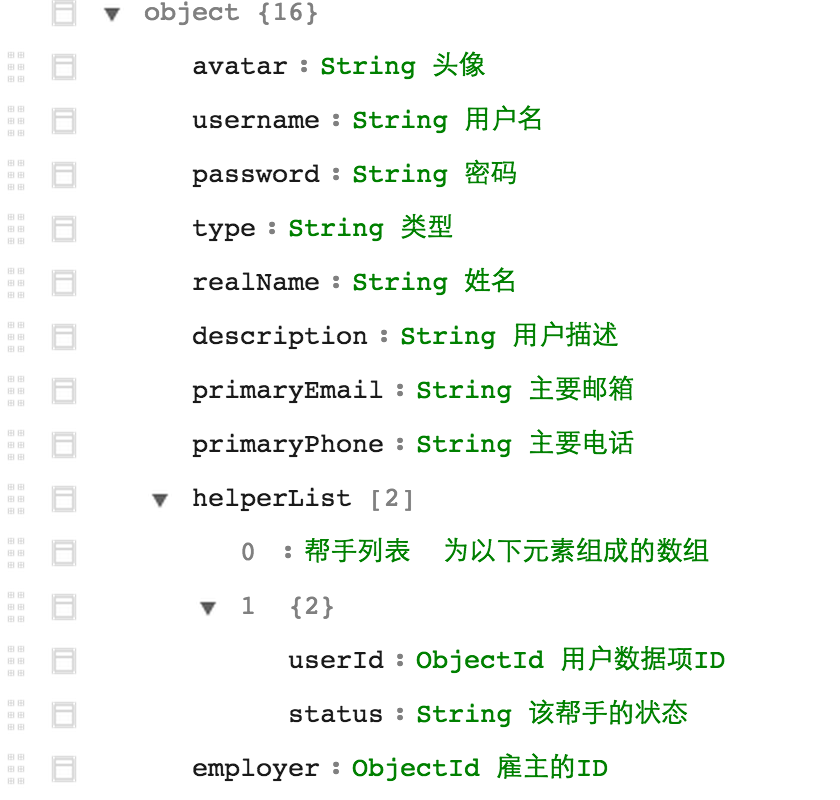
\includegraphics[width=0.45\textwidth]{user-1.png}
        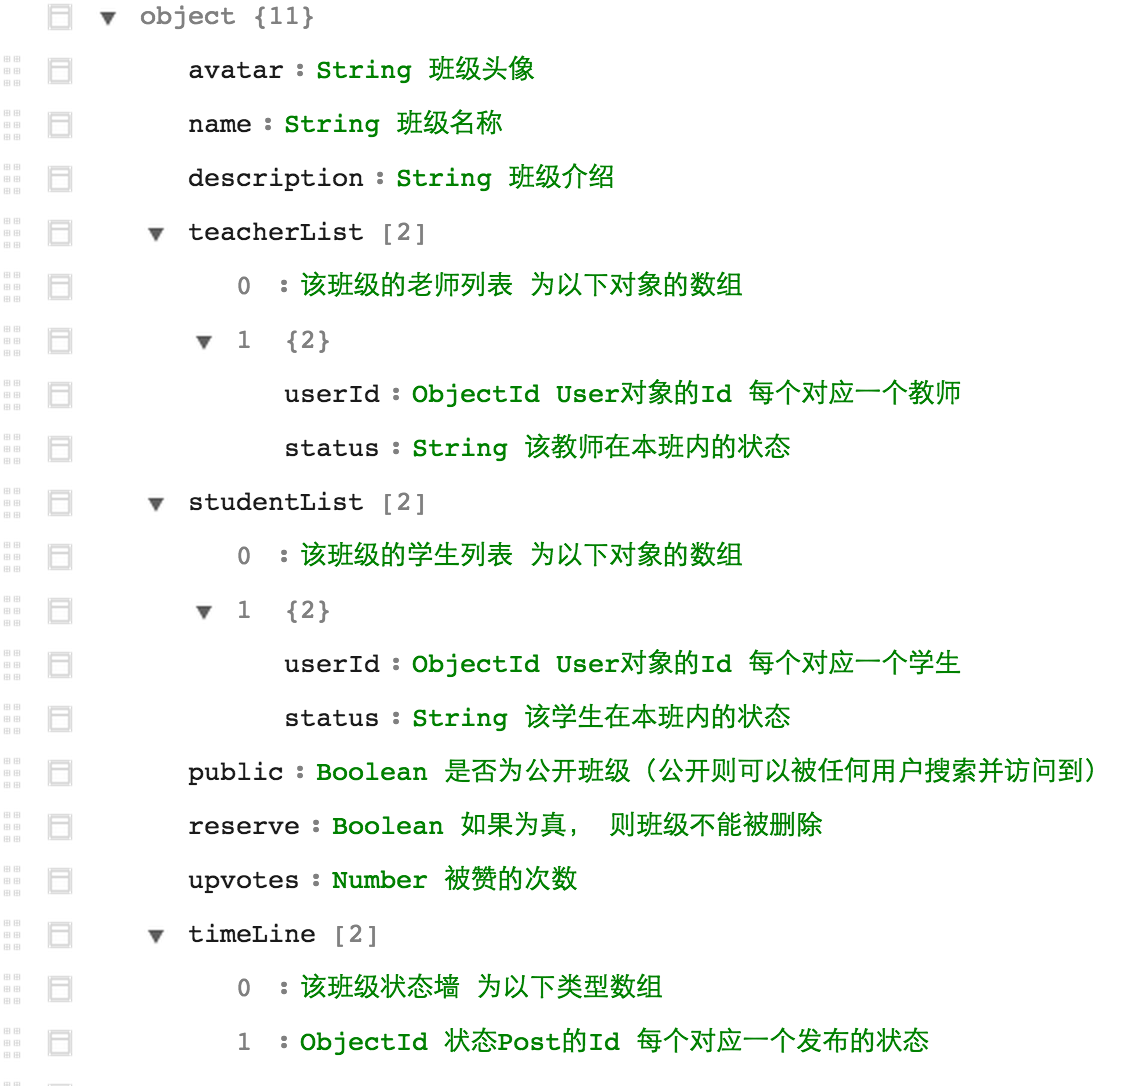
\includegraphics[width=0.45\textwidth]{user-2.png}
        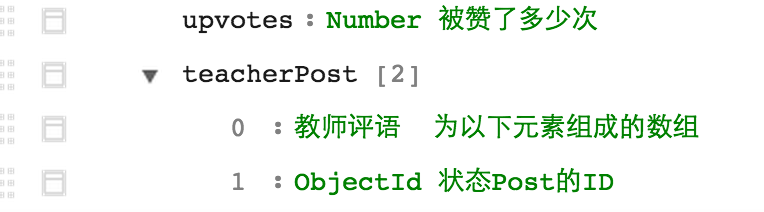
\includegraphics[width=0.45\textwidth]{user-3.png}
	\figcaption{用户模型具体定义}
	\label{fig:user-defined}
\end{figure}


\subsection{学校}


\begin{figure}[H]
	\centering
        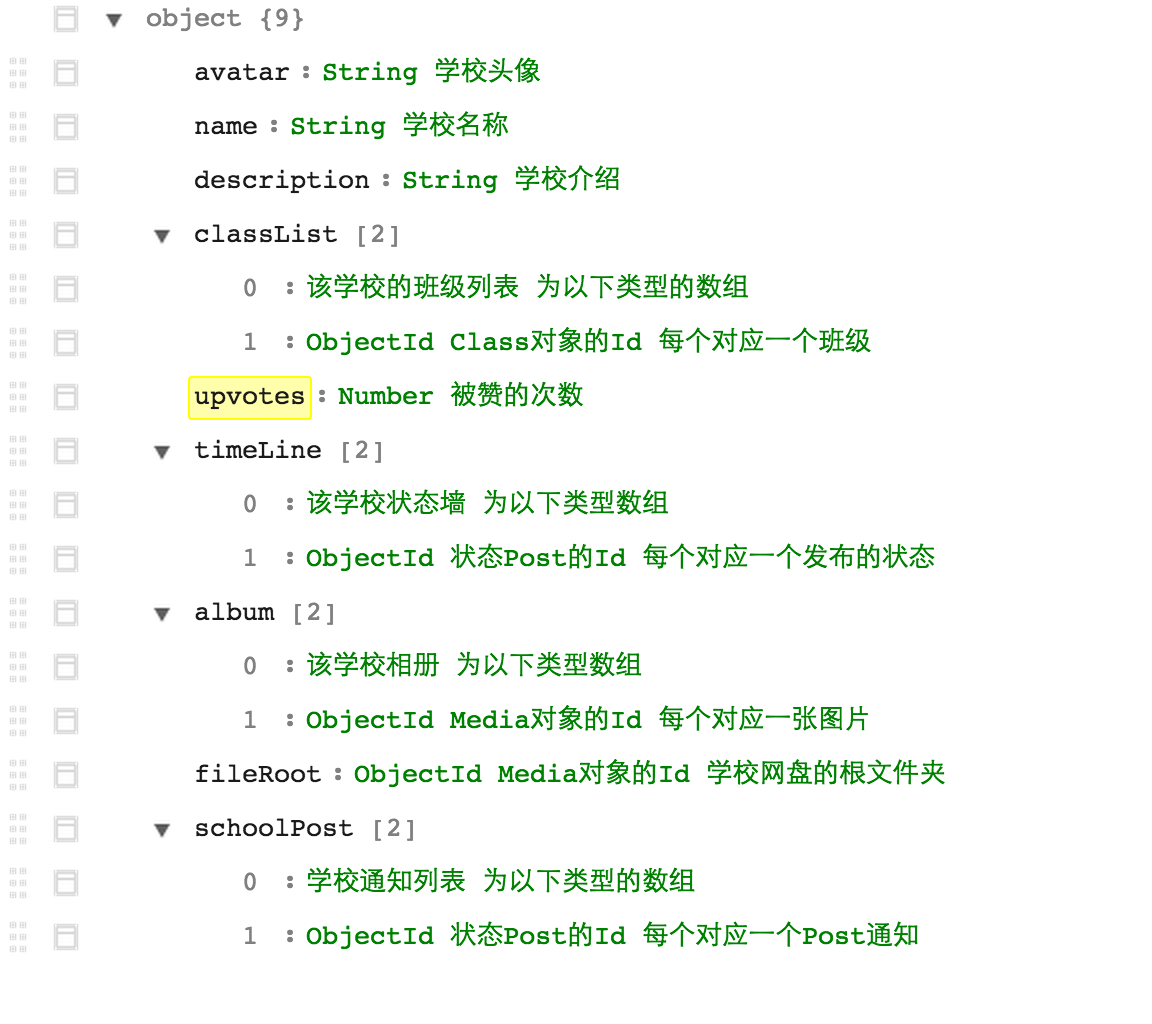
\includegraphics[width=0.8\textwidth]{school.png}
	\figcaption{学校模型具体定义}
	\label{fig:school-defined}
\end{figure}

\subsection{班级}

\begin{figure}[H]
	\centering
        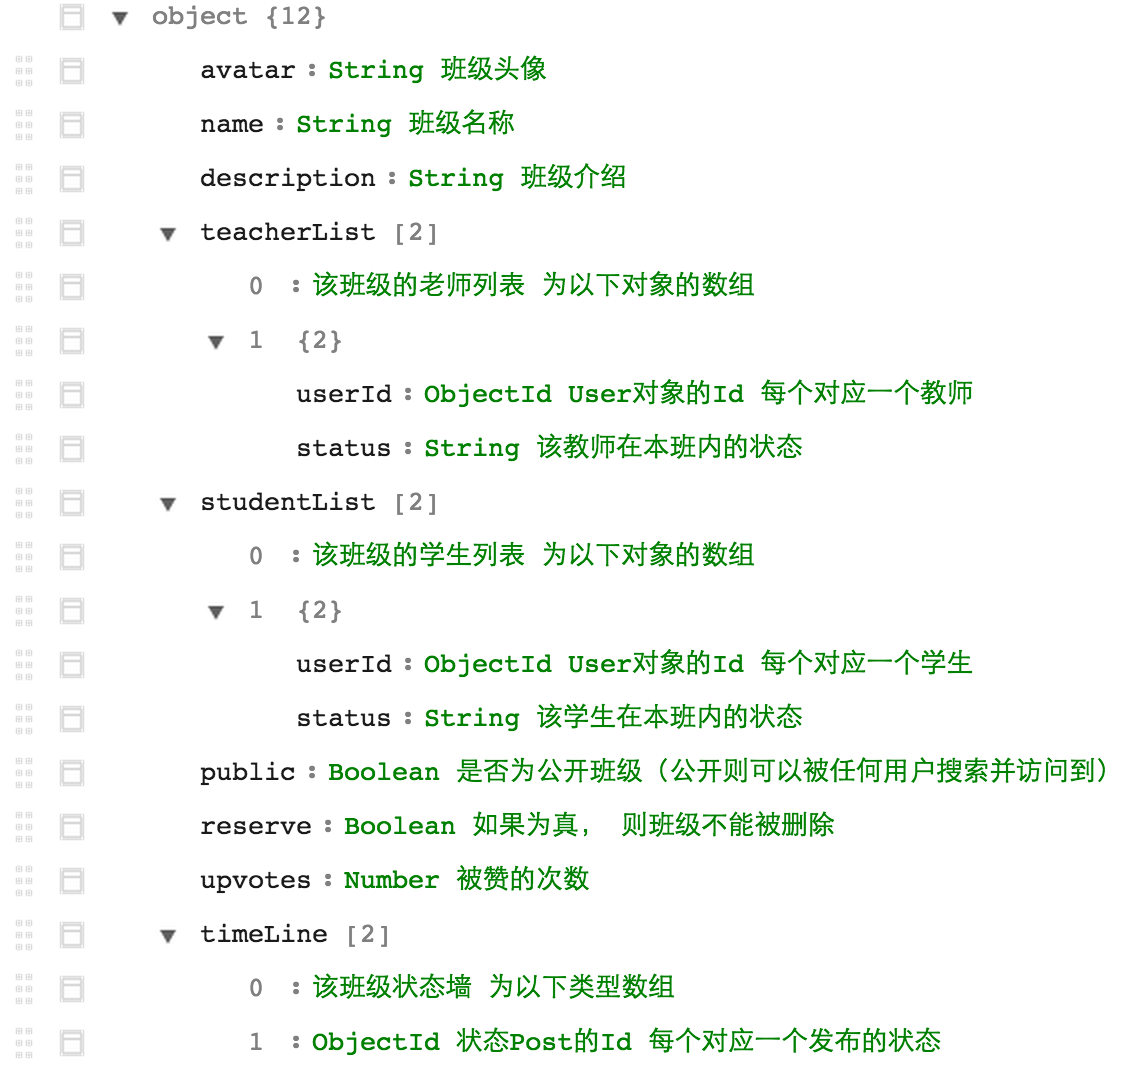
\includegraphics[width=0.45\textwidth]{class-1.png}
        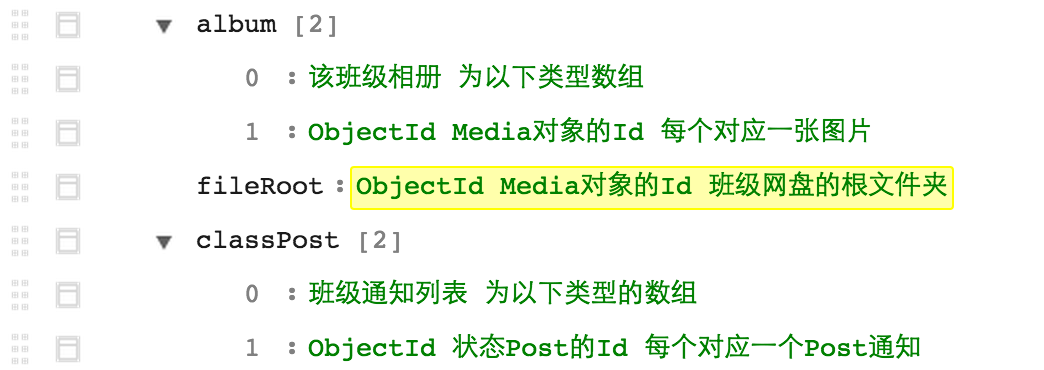
\includegraphics[width=0.45\textwidth]{class-2.png}
	\figcaption{班级模型具体定义}
	\label{fig:class-defined}
\end{figure}

\subsection{状态}

\begin{figure}[H]
	\centering
        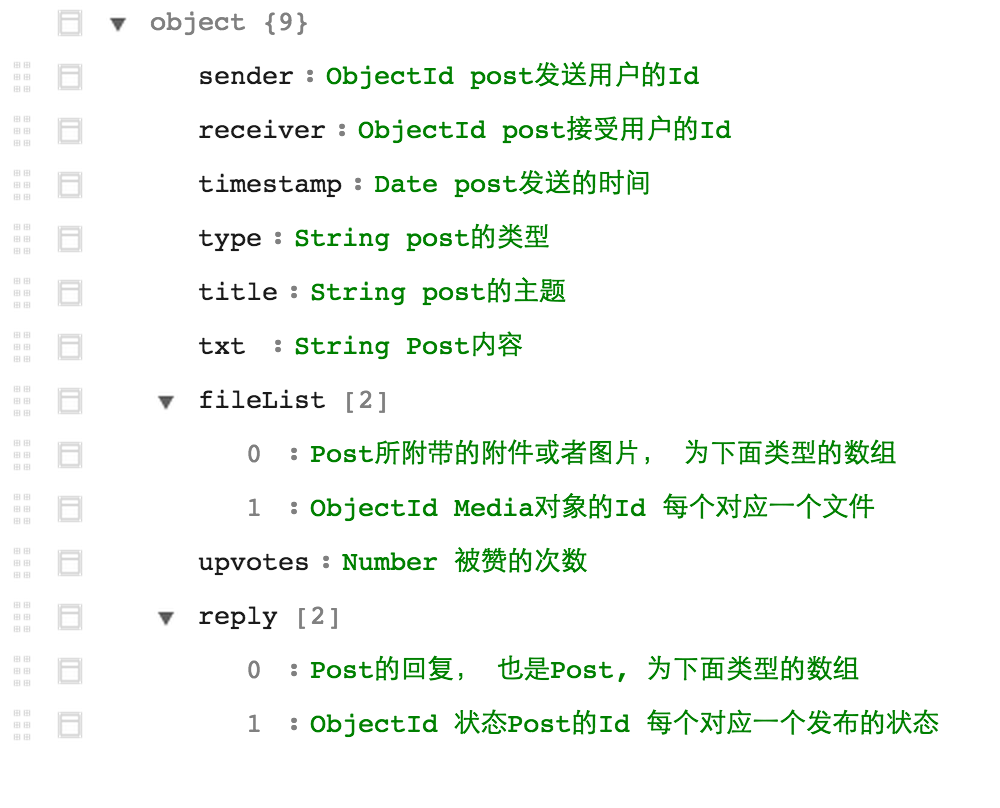
\includegraphics[width=0.8\textwidth]{post.png}
	\figcaption{状态模型具体定义}
	\label{fig:post-defined}
\end{figure}

\subsection{媒体Media (文件的存储)}

\begin{figure}[H]
	\centering
        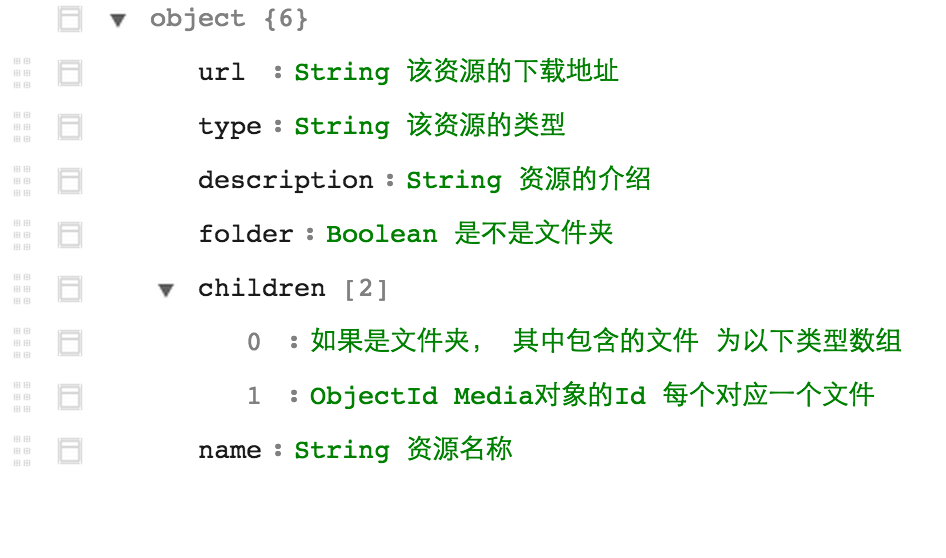
\includegraphics[width=0.8\textwidth]{media.png}
	\figcaption{文件模型具体定义}
	\label{fig:media-defined}
\end{figure}

\subsection{验证Token}

\begin{figure}[H]
	\centering
        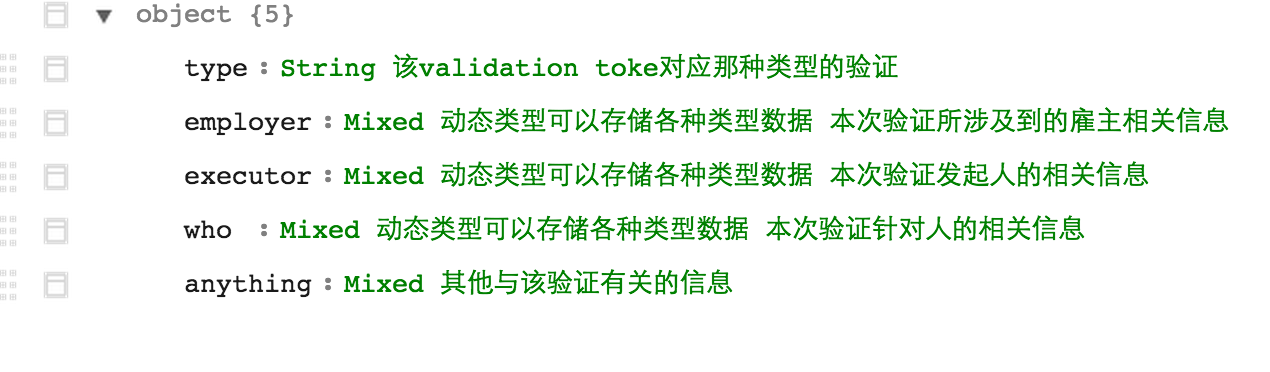
\includegraphics[width=0.8\textwidth]{validation.png}
	\figcaption{验证Token模型具体定义}
	\label{fig:validation-defined}
\end{figure}


\section{服务器端功能实现}

下面给出系统关键模块暴露出的api,和一些api的实现解释和细节

\subsection{Top Level 最上层代码}

下面给出整个app最顶层程序的伪代码


\hspace{1cm}
\begin{minipage}{1.0\linewidth}

\begin{Code}[label=index.js]
var config = require(app.config)
server = http.createServer(config.port);
socket_server = socket.io(server);
var modules  =  config.server_modules;

modules.forEach(function(module_name){
	var md = require(module_name);

	md.socket.forEach(function(obj){
		socket_server.on(obj.name, obj.function)
	});

	md.server.forEach(function(obj){
		server.inject(obj.method, obj.path, obj.function);
	});
});

server.listen(function(err){
	if(!err)
		console.log(server  started successfully.);
});
\end{Code}
\end{minipage}
\hspace{1cm}

其功能是

\begin{itemize}
\item 加载app的配置模块config
\item 根据app配置的端口创建Http服务器, 并由Http服务器创建Websocket服务器
\item 加载config中设置的要向服务器中导入的模块列表
\item 将所有加载的模块注入服务器
\item 开启服务器, app正式开始运行

\end{itemize}




\subsection{app.config模块}

里面要配置的内容为

\begin{itemize}
\item 服务器要运行哪个端口
\item 要加载的模块
\item 日志的粒度
\item 是否运行在DEBUG模式
\item 数据库的细节配置, 比如如何处理索引

\end{itemize}



\subsection{app.model模块和app.thunkify模块}

数据持久化层的定义, 前面已经说得很清楚了。

\subsection{app.log模块}

是app的日志模块, 对于一个web app来说, 日志记录非常重要。 日志记录有以下作用:

\begin{enumerate}
\item  检测黑客对于服务器攻击
\item 记录用户对于app的错误使用, 方便下一版本修改
\item 记录用户使用app的习惯, 用于更好的设计产品
\item 记录服务器出的错误,找出bug
\end{enumerate}



在该app中, 我记录日志的方法为:

\begin{quote}
  先写在一个文件中, 之后用一个定时运行的程序, 把该文件所有内容写入数据库。作为数据的持久化。
\end{quote}


记录日志的种类为:

\begin{itemize}
\item DEBUG 调试信息
\item TRACE 也是只有调试的时候会用,细节信息, 比如进入了哪个函数等等
\item ERROR 发生的系统错误
\item WARN  系统的警告, 比如疑似的攻击
\item INFO  用户操作的记录
\end{itemize}





\subsection{app.privilege模块}

该模块管理系统提供了管理教师用户的权限机制

分为:
\begin{itemize}
\item HumanResource 可以管理班级内的人员
\item InfoManager 可以在任何班级和自己雇主的学校发布通知, 和修改班级, 学校介绍
\item BOSS 拥有所有权限(不只是上面的两种操作, 比如学校名称的修改)
\end{itemize}

通过或操作来完成权限的相加, 与非操作来完成权限的相减。



\subsection{app.notice模块}

使用了sendcloud.sohu.com和极光推送的服务, 完成发短信,发邮件通知和手机端Push Notification的功能。

需要通知的操作一般为:

\begin{itemize}
\item 人员的转班, 邀请等等
\item 手机端聊天的提醒
\item 忘记密码
\end{itemize}




\subsection{app.data命名空间}

在空间下, 是对于底层数据定义的抽象层

\subsubsection{class班级和school学校}

\begin{itemize}
\item 提供学校班级的创建,修改,删除
\item 这里删除使用软删除,不真正删除数据而是用一个Deleted的布尔标记
\item 人员转班转校
\end{itemize}

\subsubsection{post状态}

\begin{itemize}
\item 发送状态
\item 删除所发状态
\end{itemize}

\subsubsection{file文件和image图片}

\begin{itemize}
\item 文件的删除,修改, 新建
\item 文件夹的展开
\item 删除依旧使用软删除
\item 相册是一个只有一层的文件夹
\end{itemize}



\subsubsection{app.validationToken模块}

处理申请request操作


\begin{itemize}
\item 比如用户提交转班,邀请某人加入某班的申请, 该模块会创建一个validationToken

\item validationToken创建的时候, 会执行验证的Pre函数, 该函数会根据该Token的类型, 来执行验证的预操作, 比如改变用户的状态。

\item 当用户点击验证连接同意验证的时候, 该模块会根据Token的类型, 执行Post函数, 完成验证的后续操作, 真正改变用户班级归属。
\end{itemize}





\section{Web管理端界面设计}

\begin{itemize}

\item 学校信息界面

\begin{figure}[H]
  \centering
  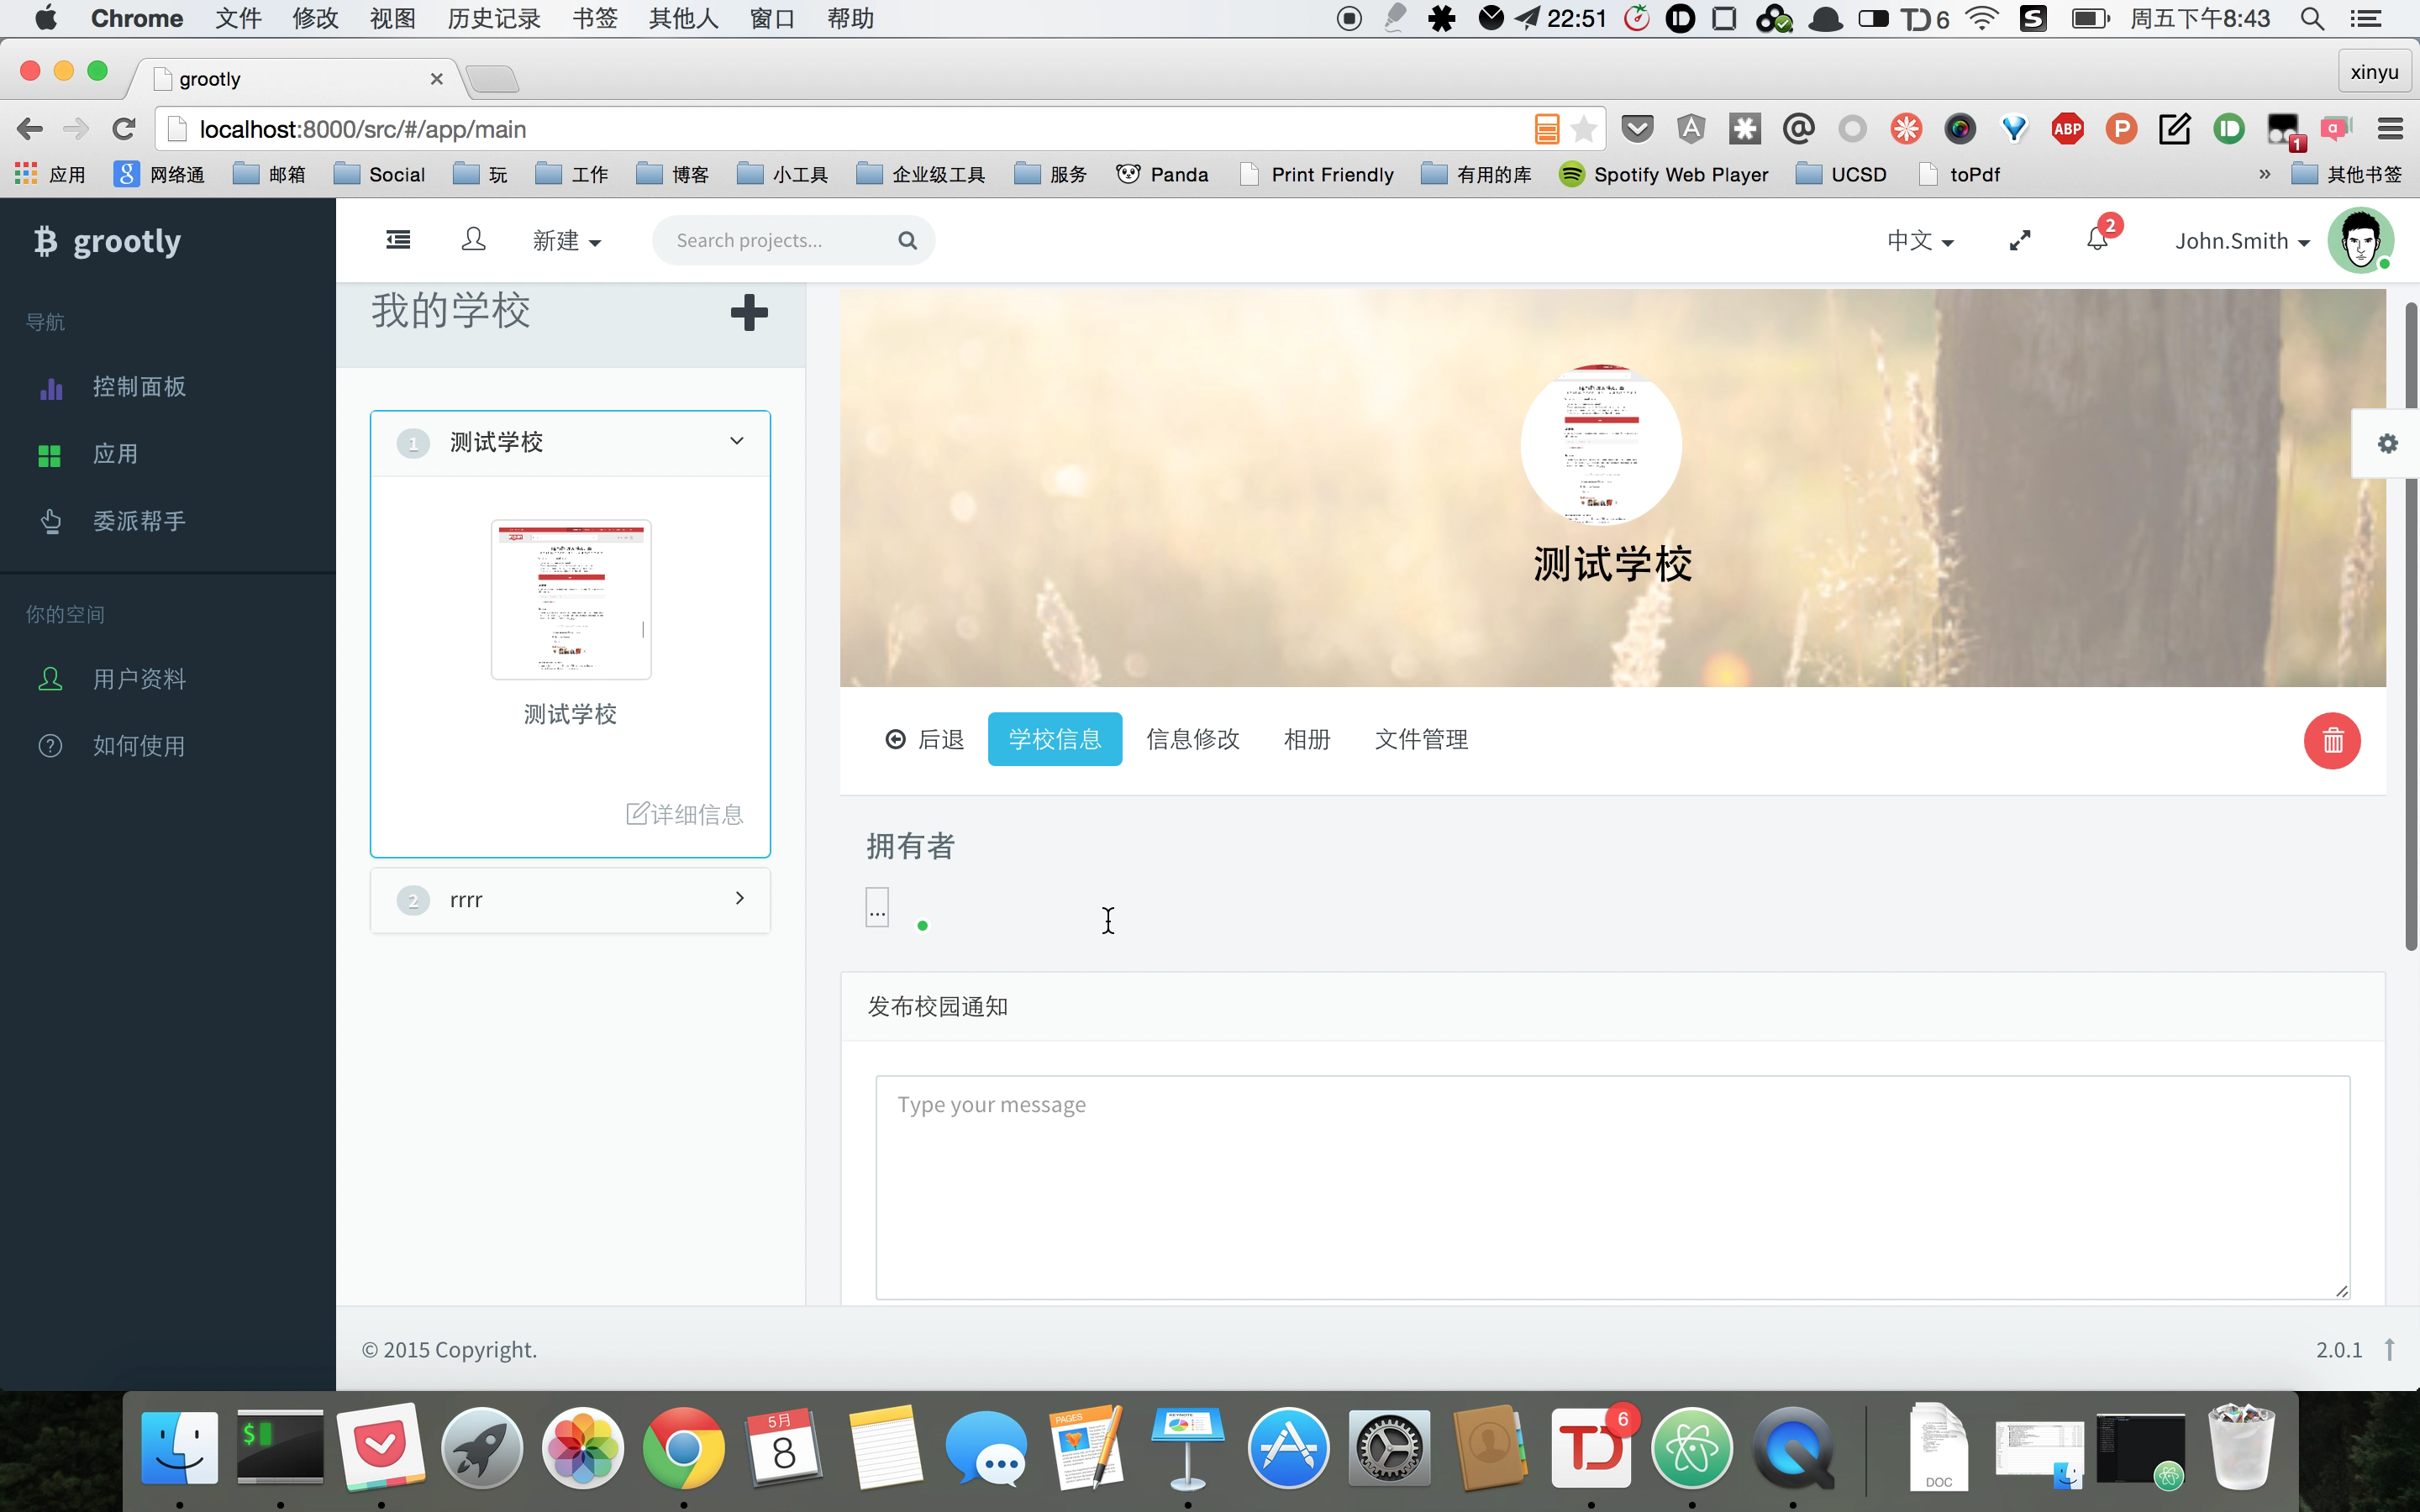
\includegraphics[width=0.7\textwidth]{school_page.png}
  \figcaption{Web管理端 学校信息界面}
  \label{fig: pc_schoolinfo}
\end{figure}


\item 班级列表界面

\begin{figure}[H]
  \centering
  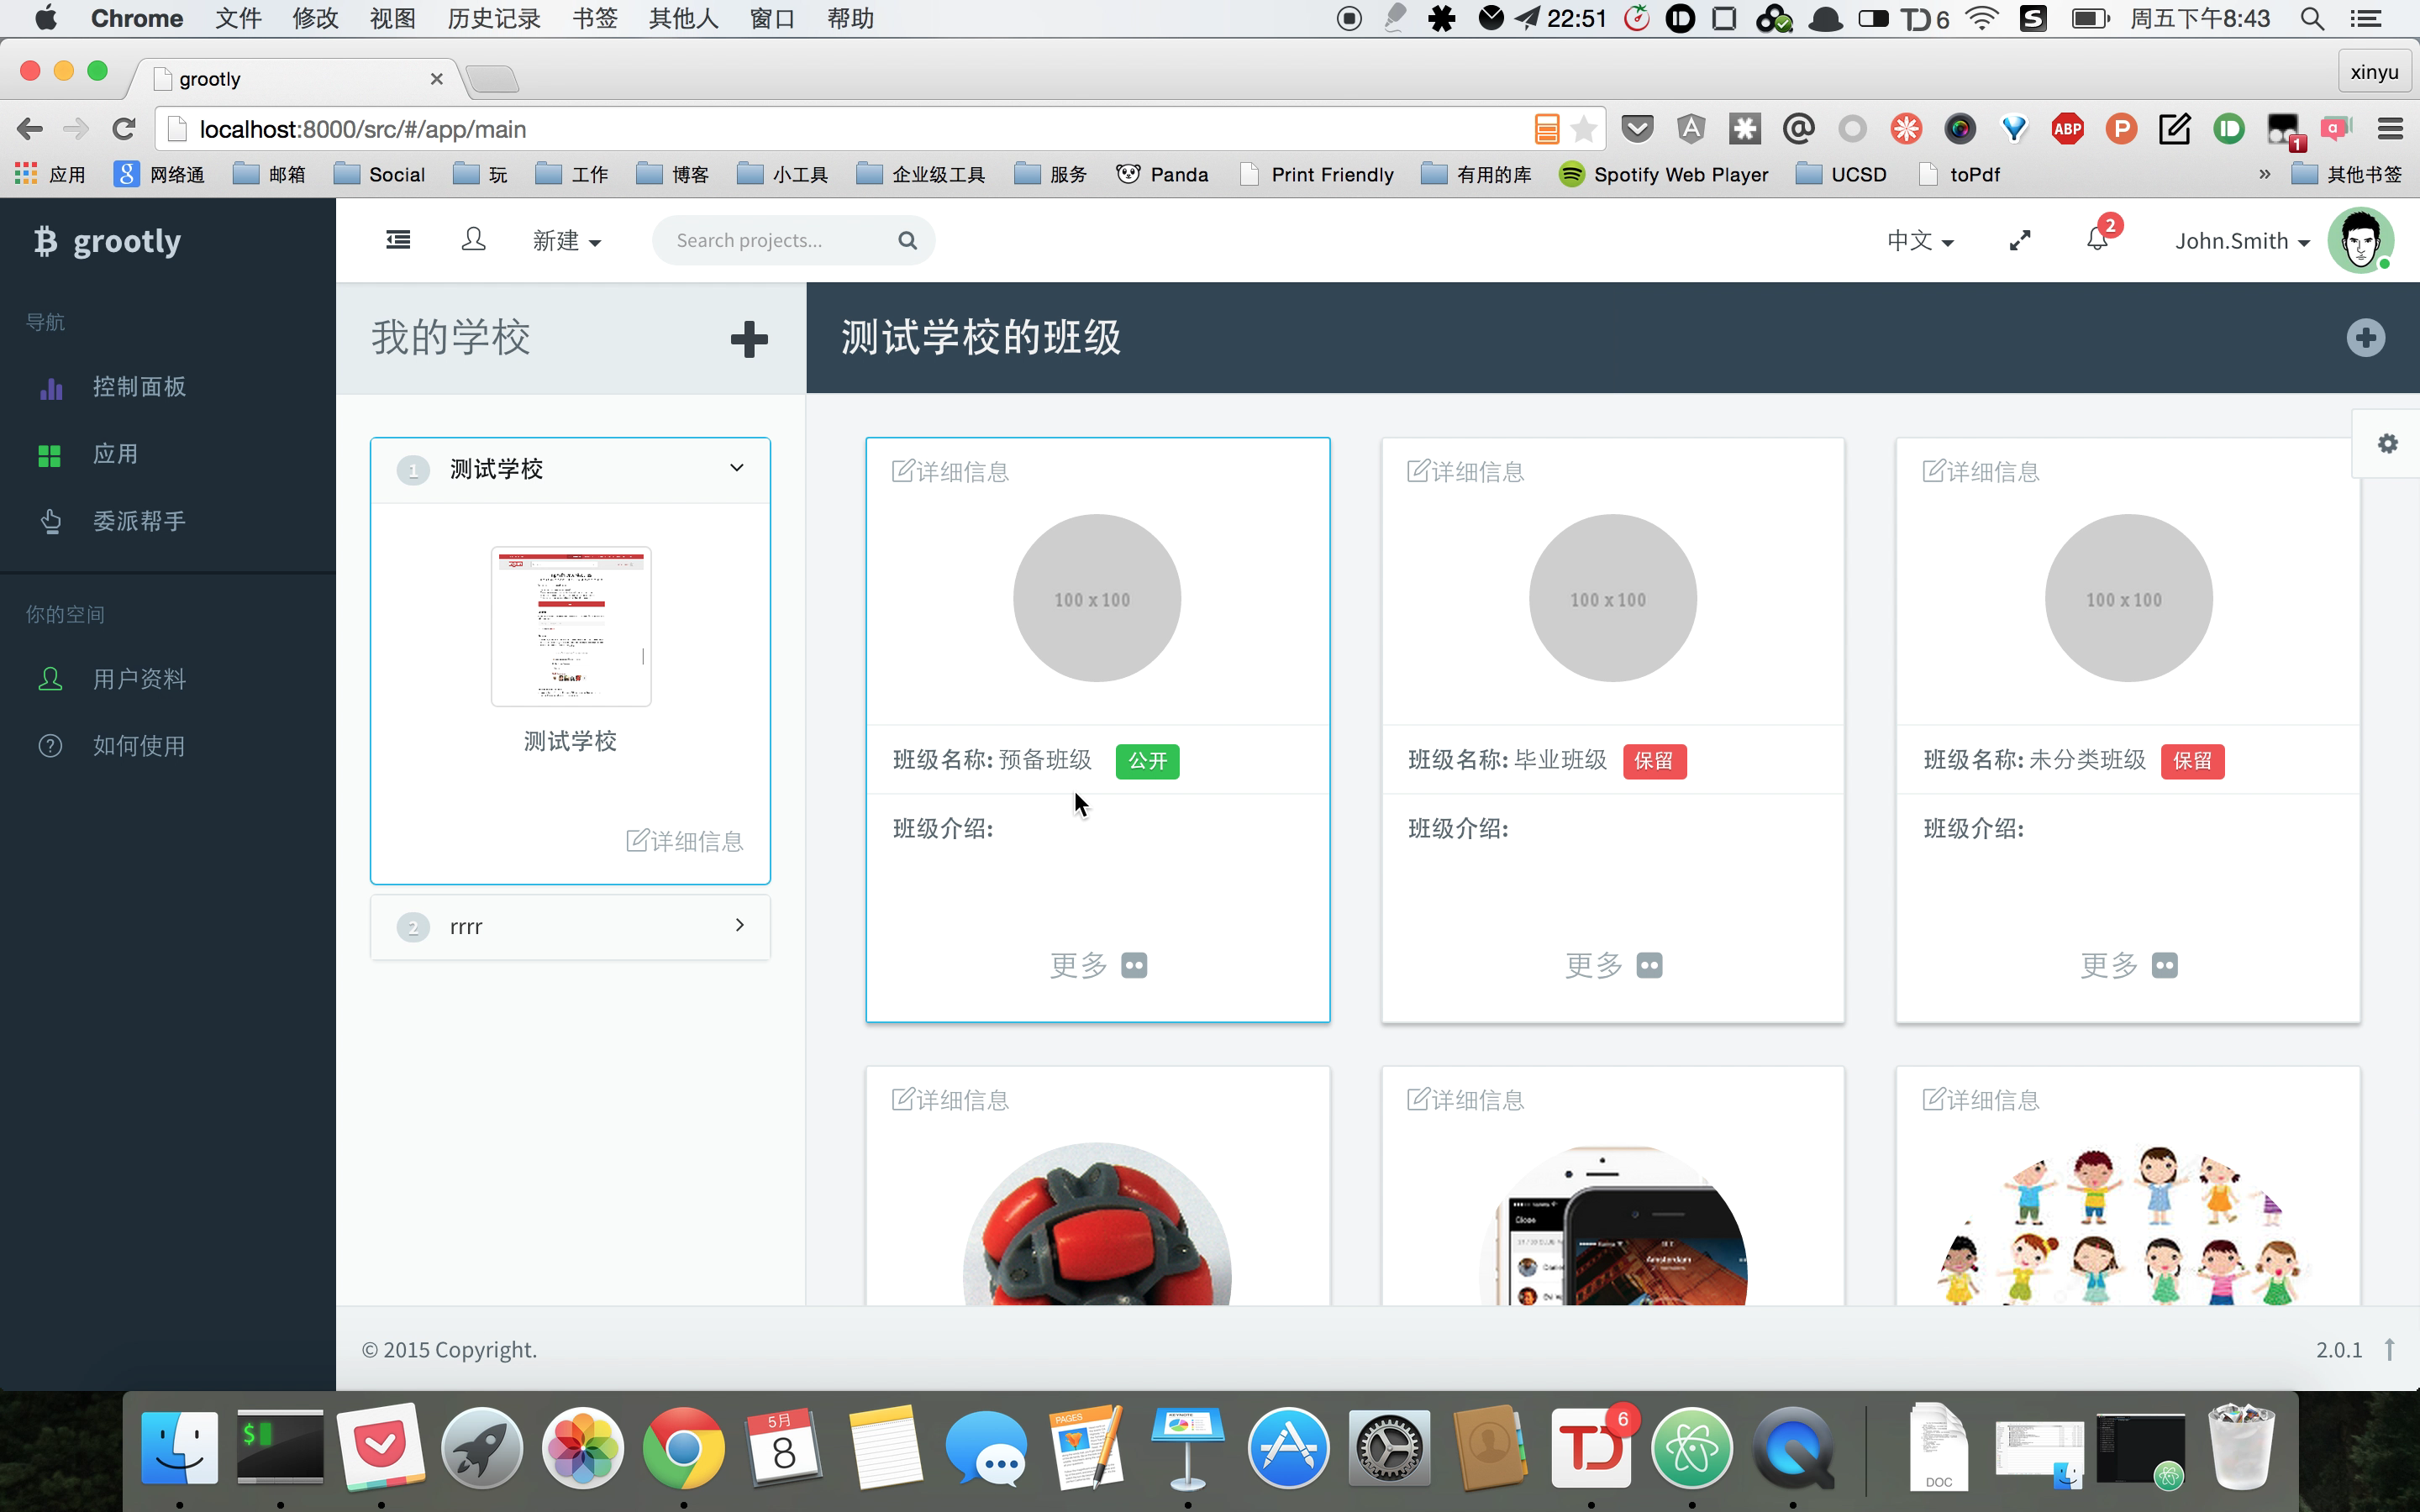
\includegraphics[width=0.7\textwidth]{my_class_list.png}
  \figcaption{Web管理端 班级列表界面}
  \label{fig: pc_classlist}
\end{figure}


\item 网盘界面

\begin{figure}[H]
  \centering
  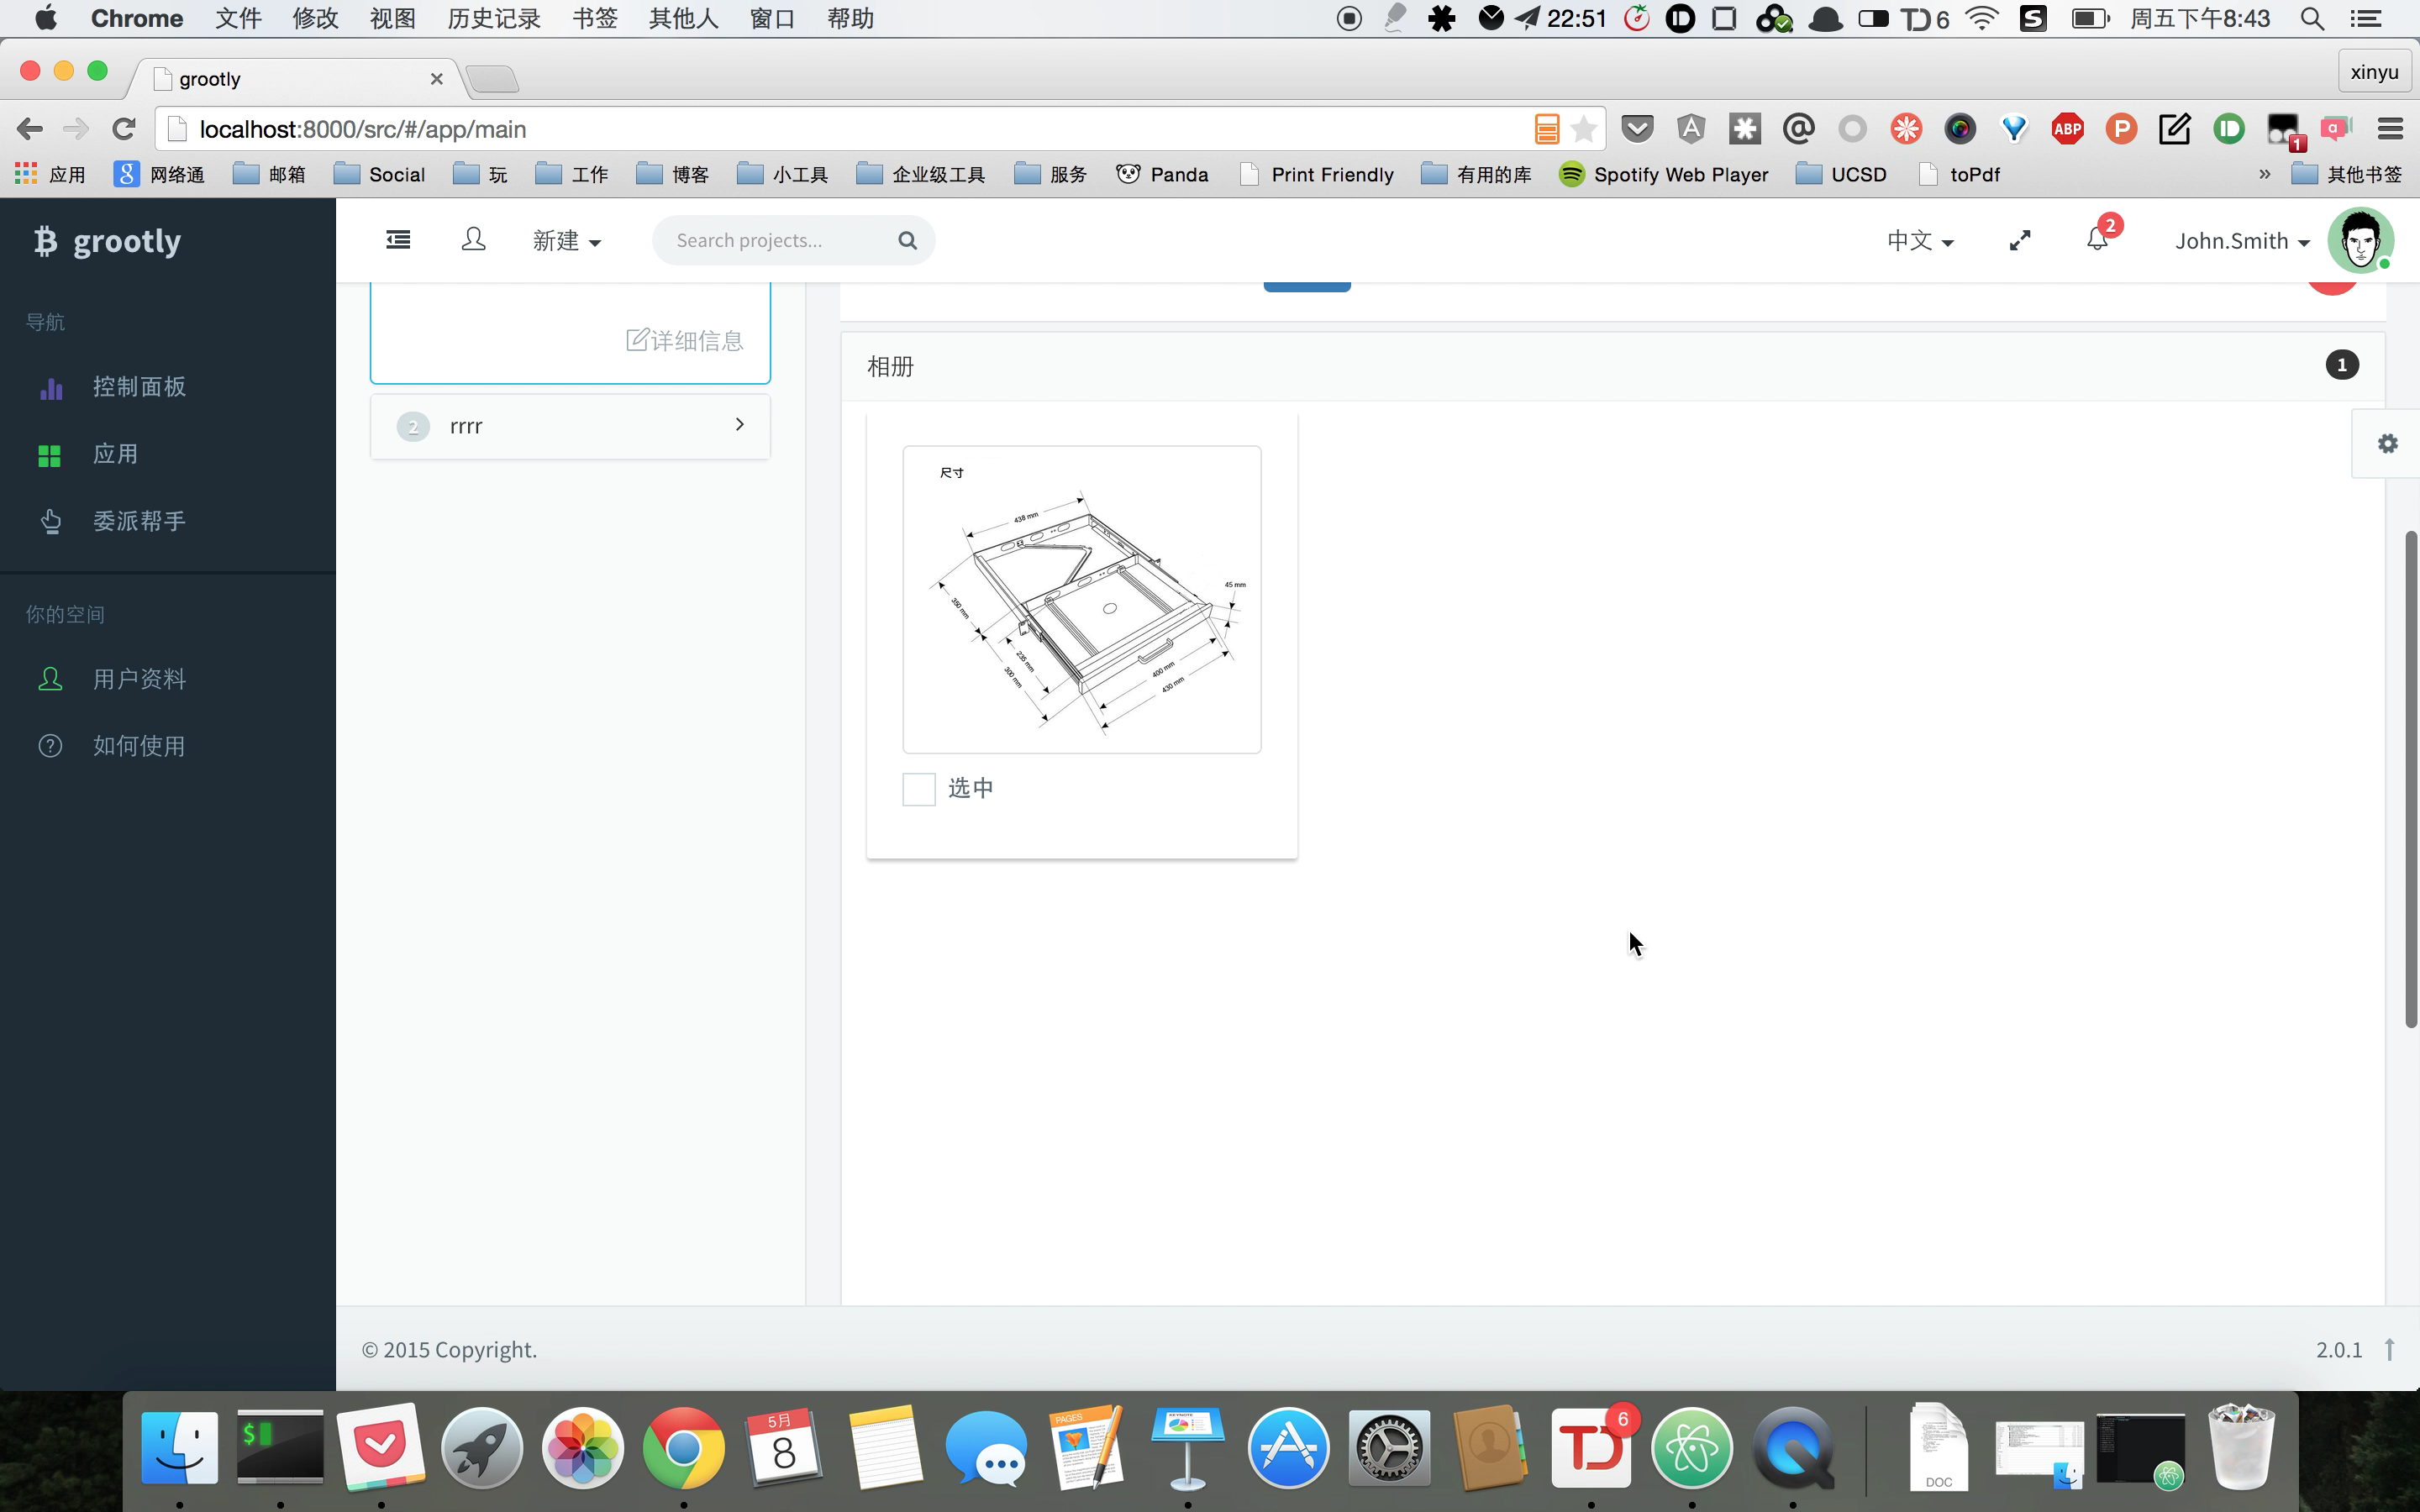
\includegraphics[width=0.7\textwidth]{album1.png}
  \figcaption{Web管理端 相册界面1}
  \label{fig: pc_album1}
\end{figure}



\begin{figure}[H]
  \centering
  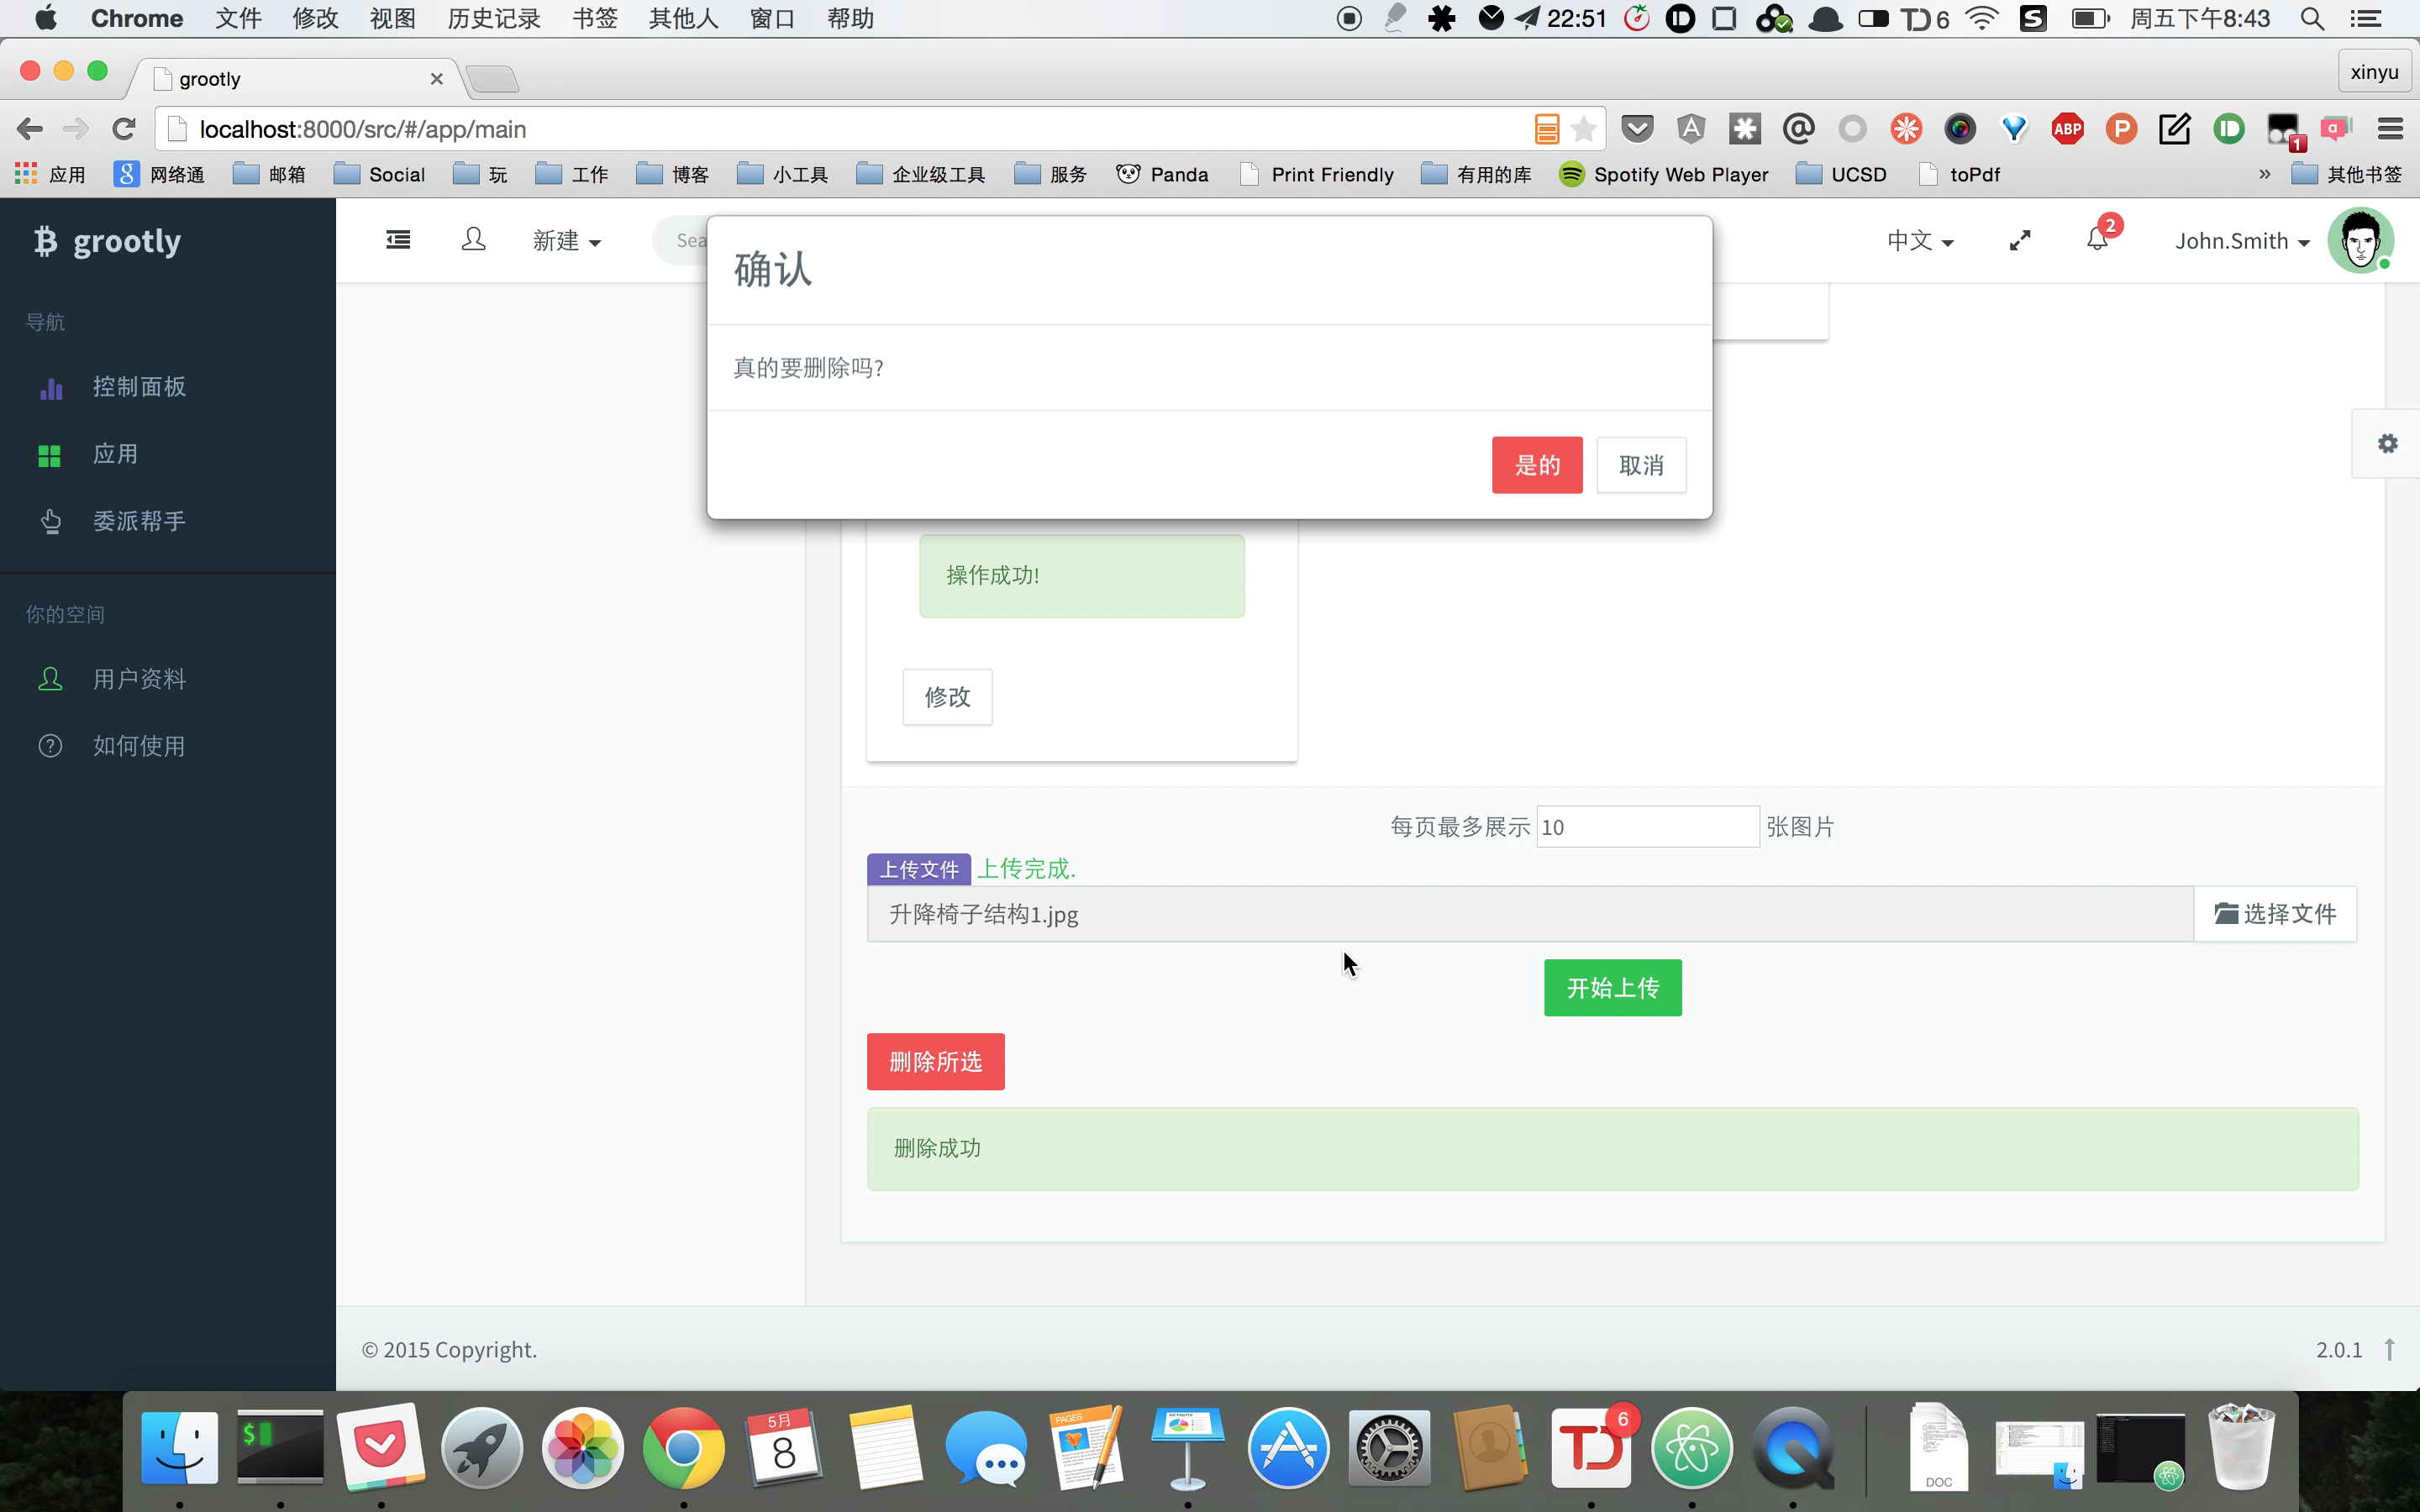
\includegraphics[width=0.7\textwidth]{album2.png}
  \figcaption{Web管理端 相册界面2}
  \label{fig: pc_album2}
\end{figure}


\item 相册界面

\begin{figure}[H]
  \centering
  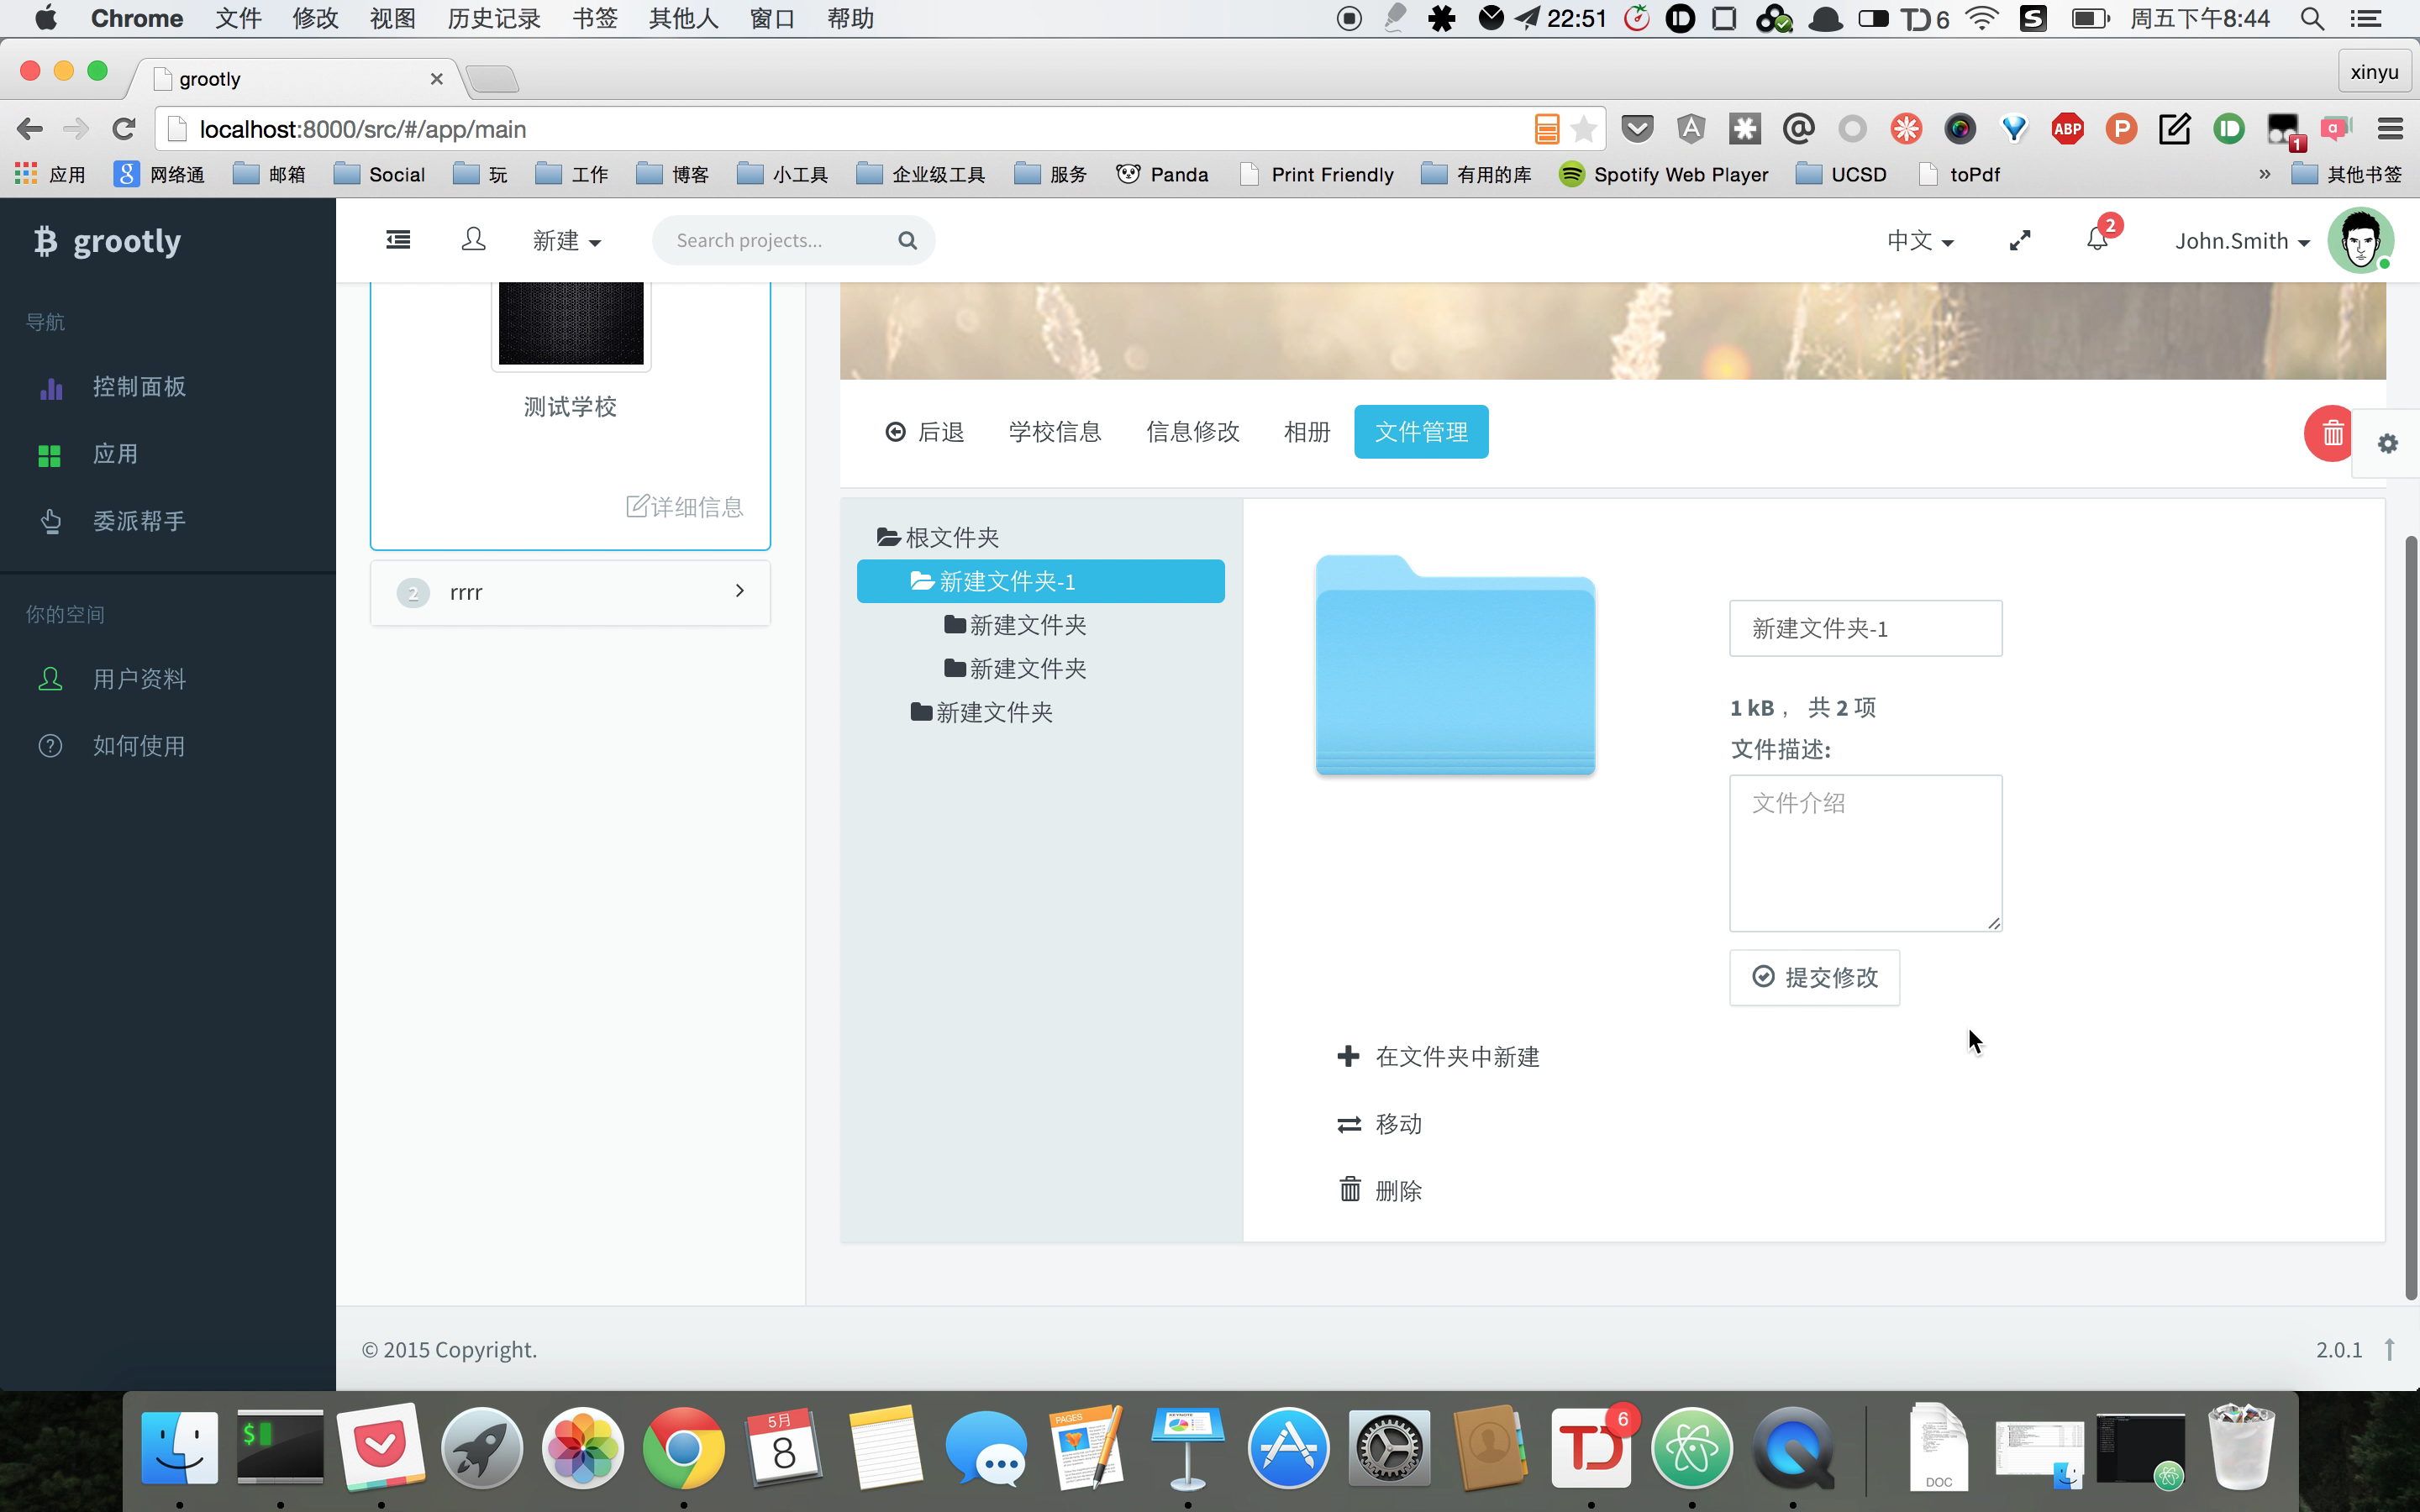
\includegraphics[width=0.7\textwidth]{pan1.png}
  \figcaption{Web管理端 网盘界面1}
  \label{fig: pc_pan1}
\end{figure}



\begin{figure}[H]
  \centering
  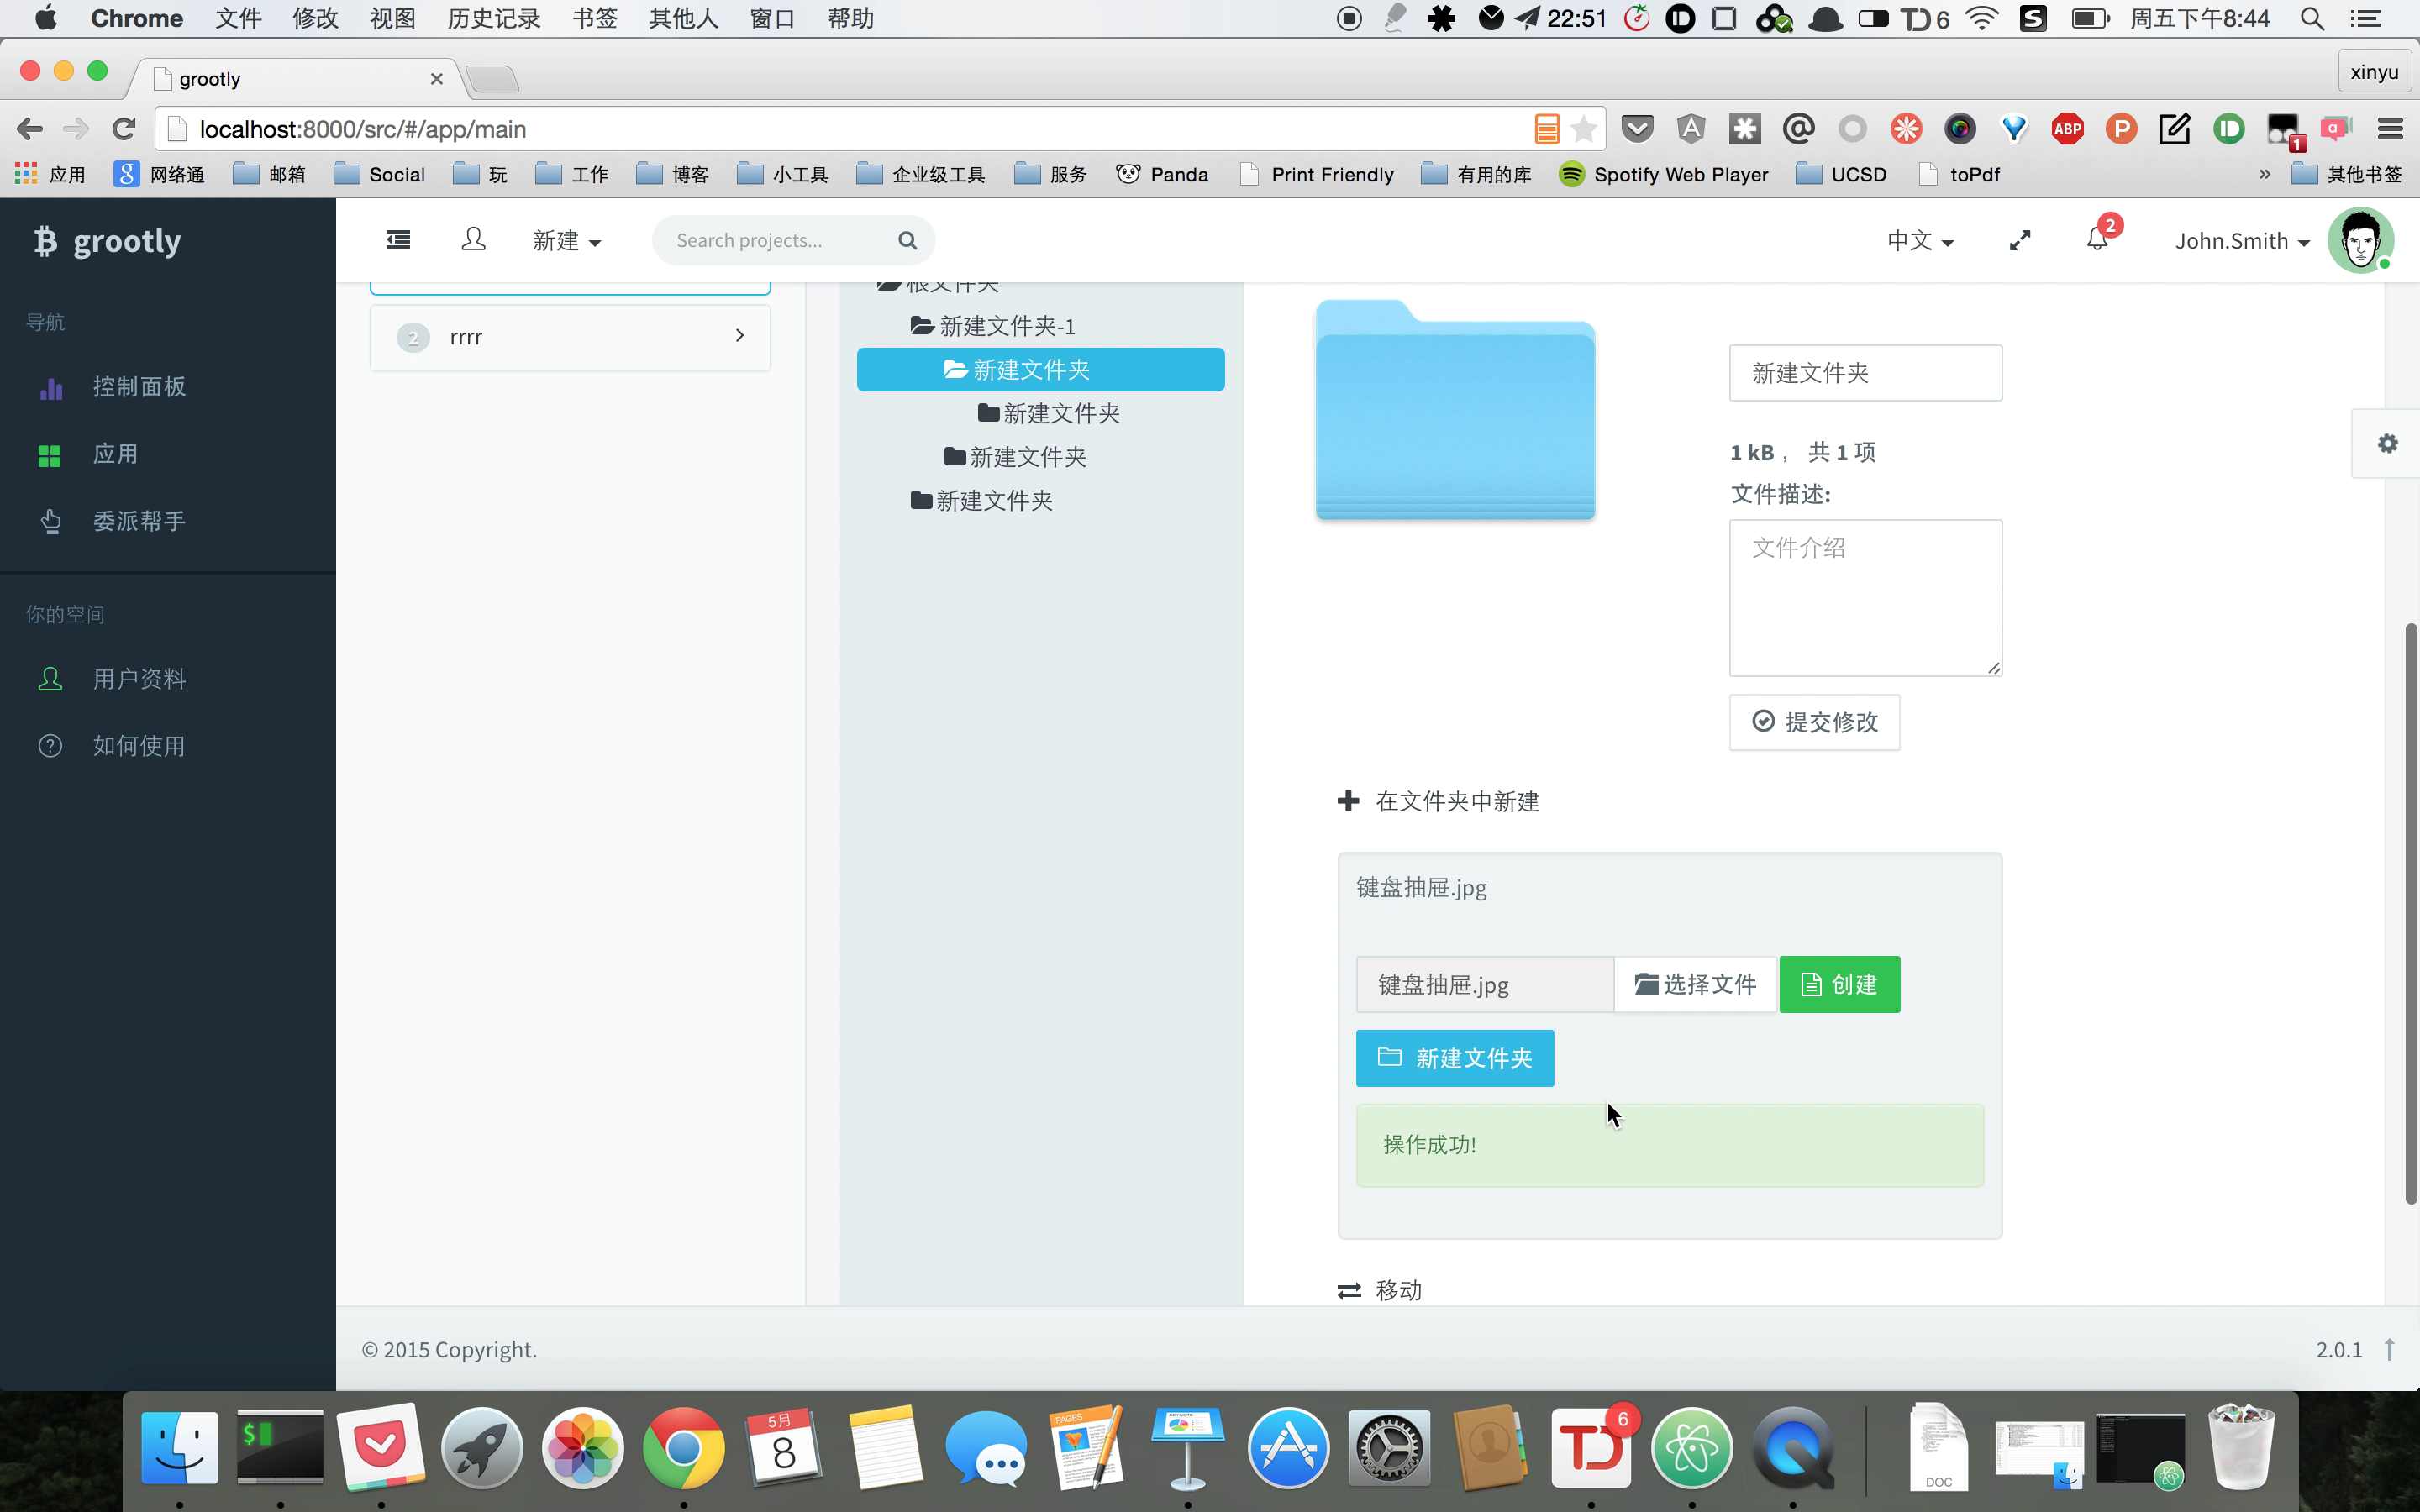
\includegraphics[width=0.7\textwidth]{pan2.png}
  \figcaption{Web管理端 网盘界面2}
  \label{fig: pc_pan2}
\end{figure}



\item 教师,学生的管理界面

\begin{figure}[H]
  \centering
  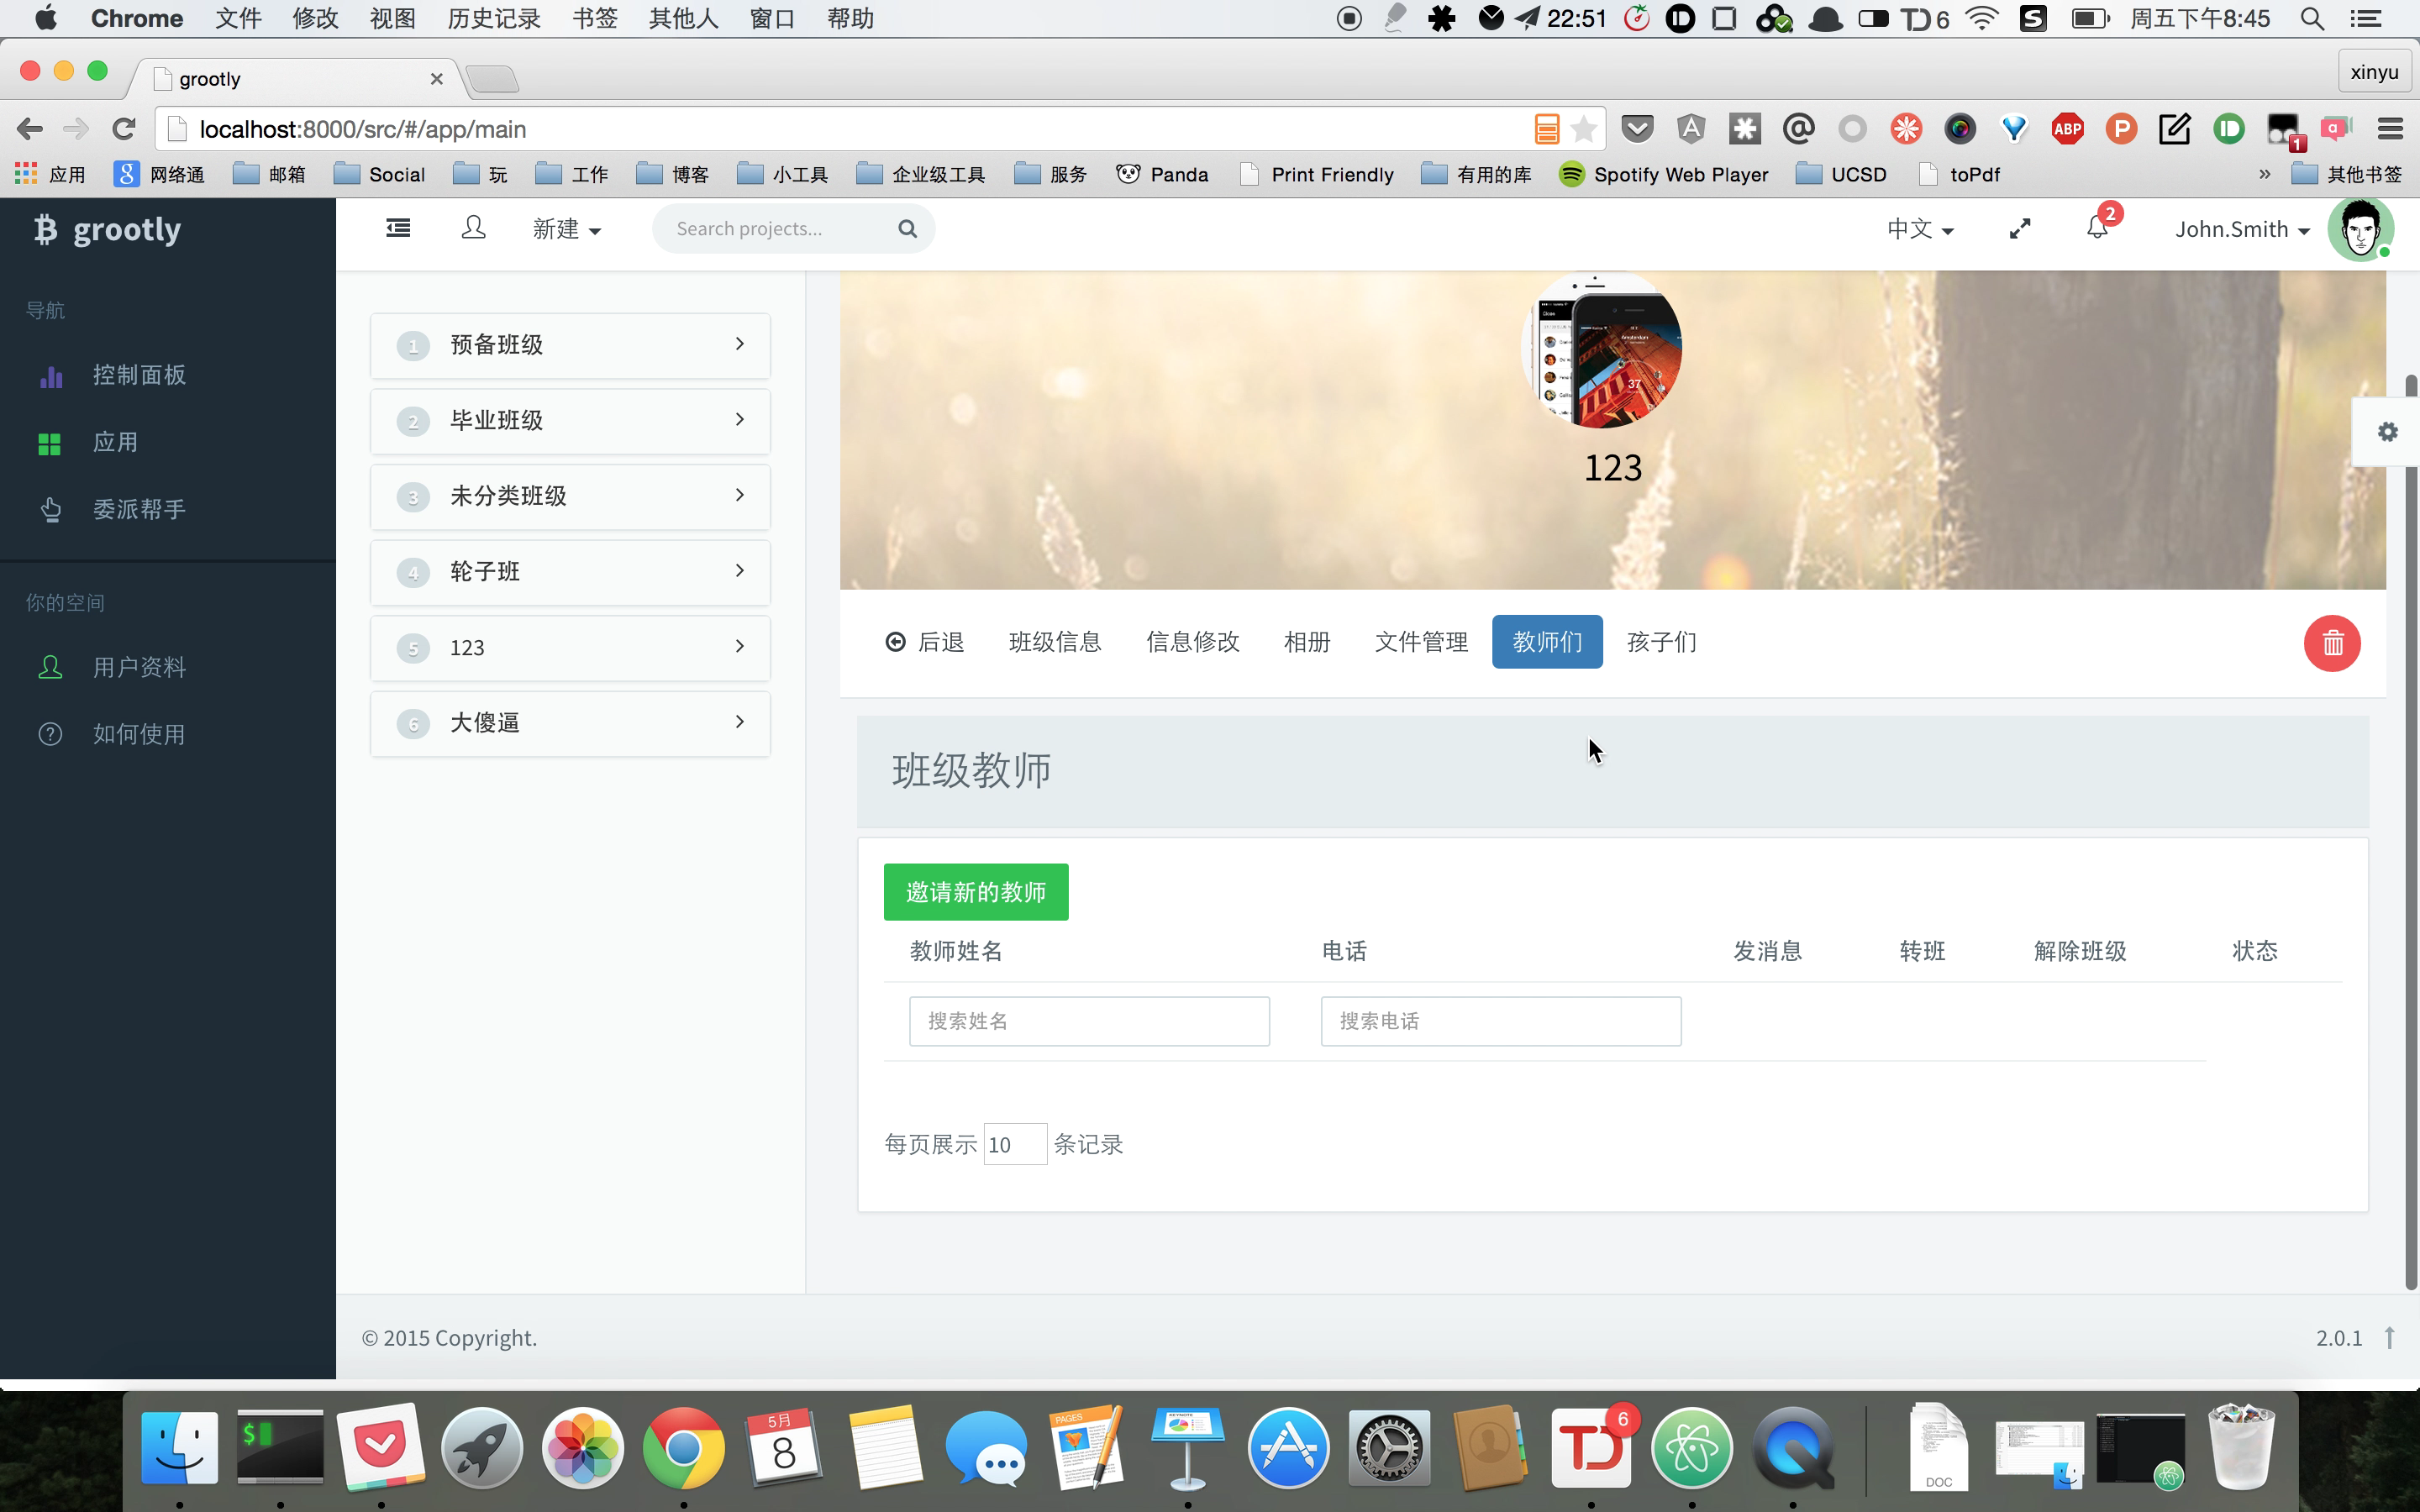
\includegraphics[width=0.7\textwidth]{my_teacher.png}
  \figcaption{Web管理端 教师列表界面}
  \label{fig: pc_my_teacher}
\end{figure}


\begin{figure}[H]
  \centering
  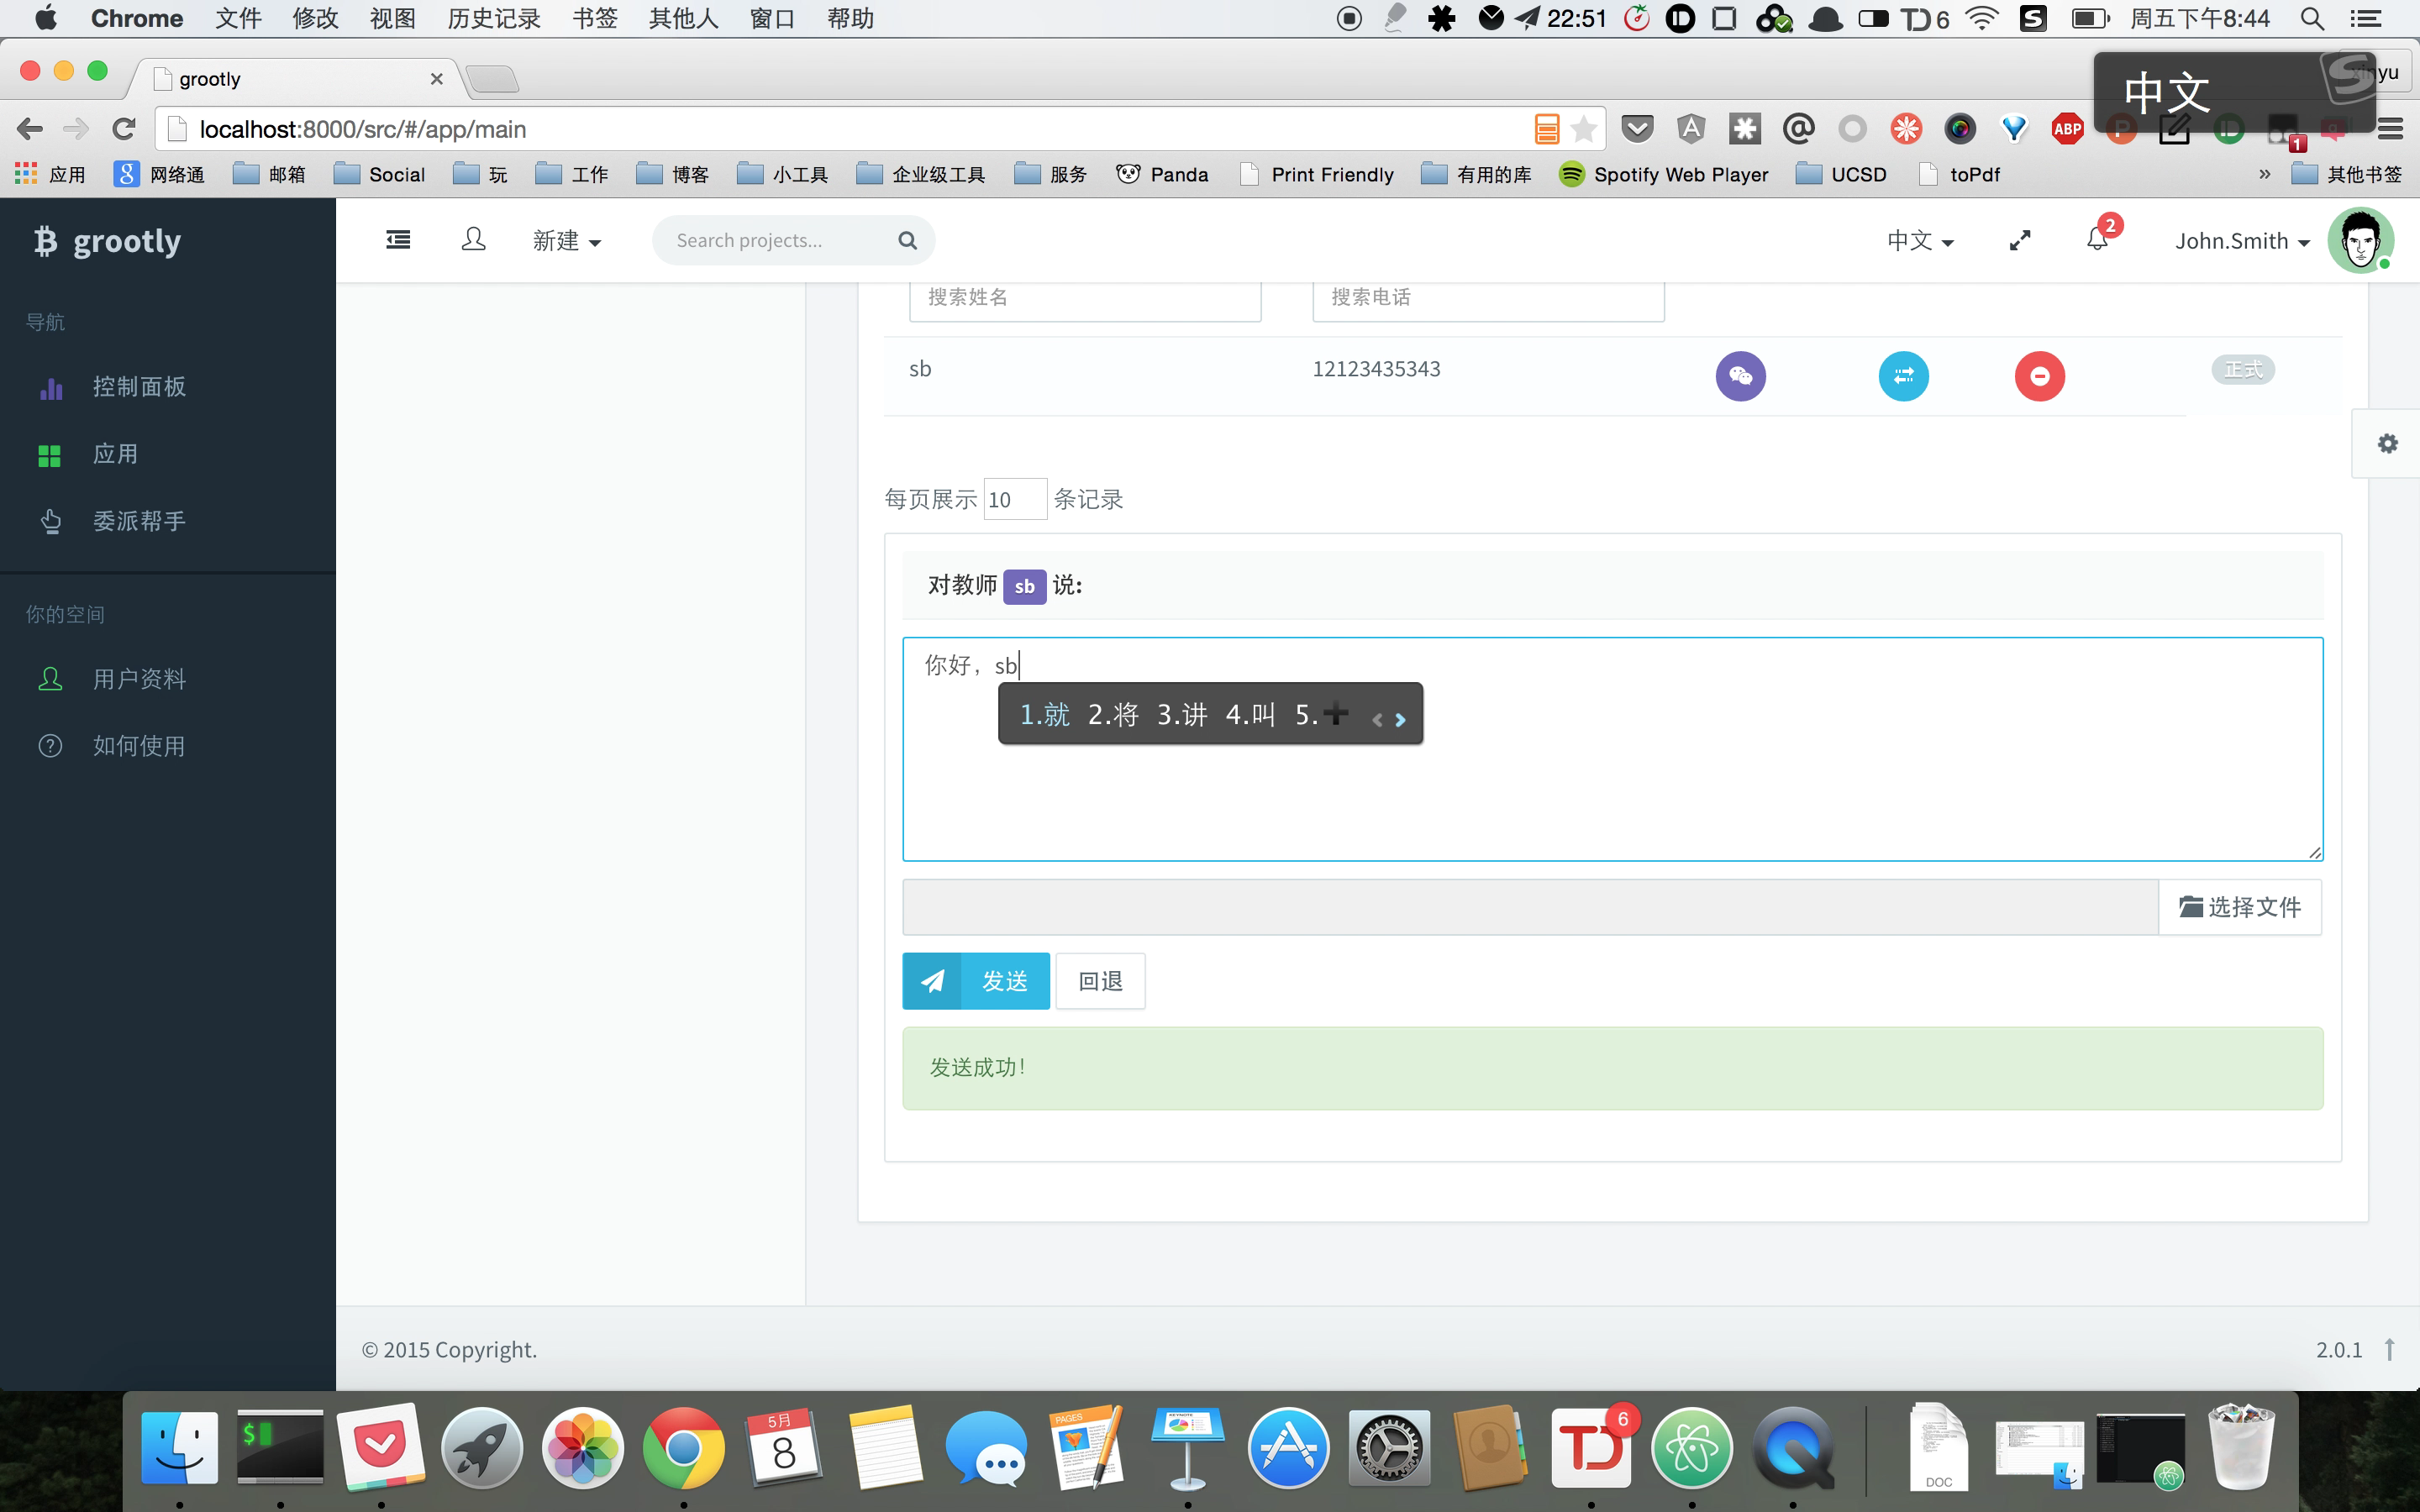
\includegraphics[width=0.7\textwidth]{people_post.png}
  \figcaption{Web管理端 人员发布通知界面}
  \label{fig: pc_people_post}
\end{figure}

\begin{figure}[H]
  \centering
  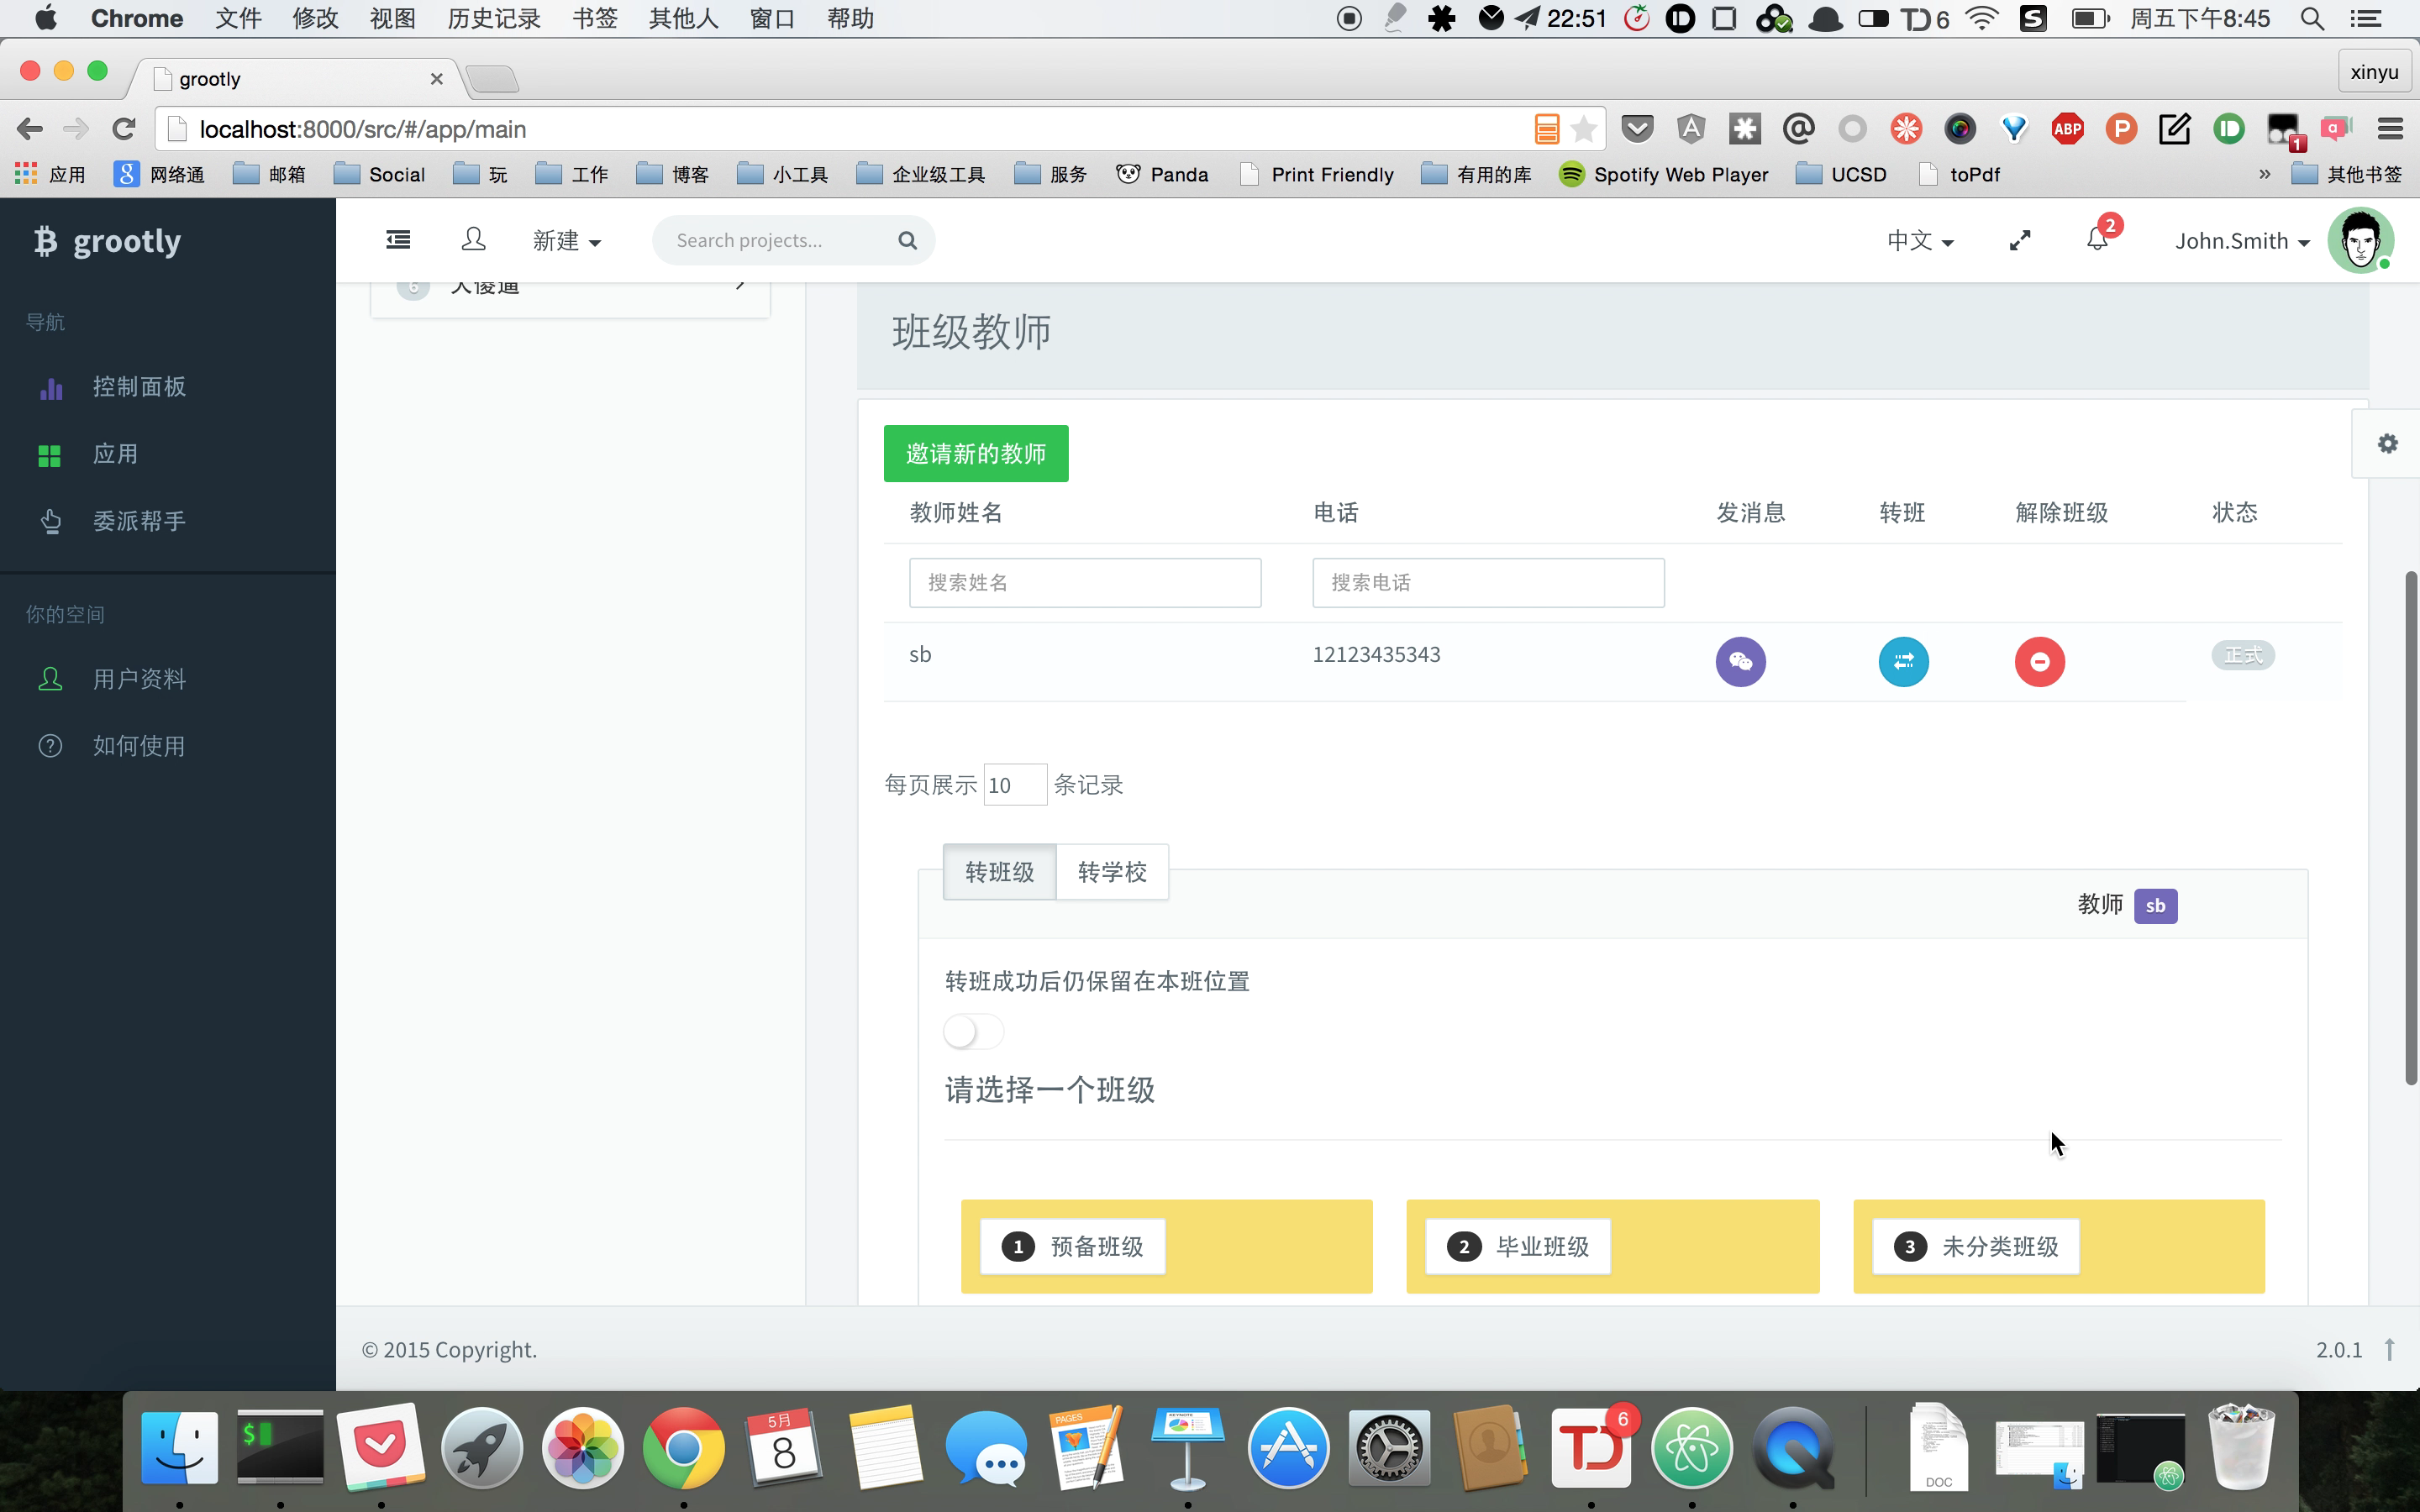
\includegraphics[width=0.7\textwidth]{people_transfer.png}
  \figcaption{Web管理端 人员转班界面}
  \label{fig: pc_people_transfer}
\end{figure}


\item 帮手界面

\begin{figure}[H]
  \centering
  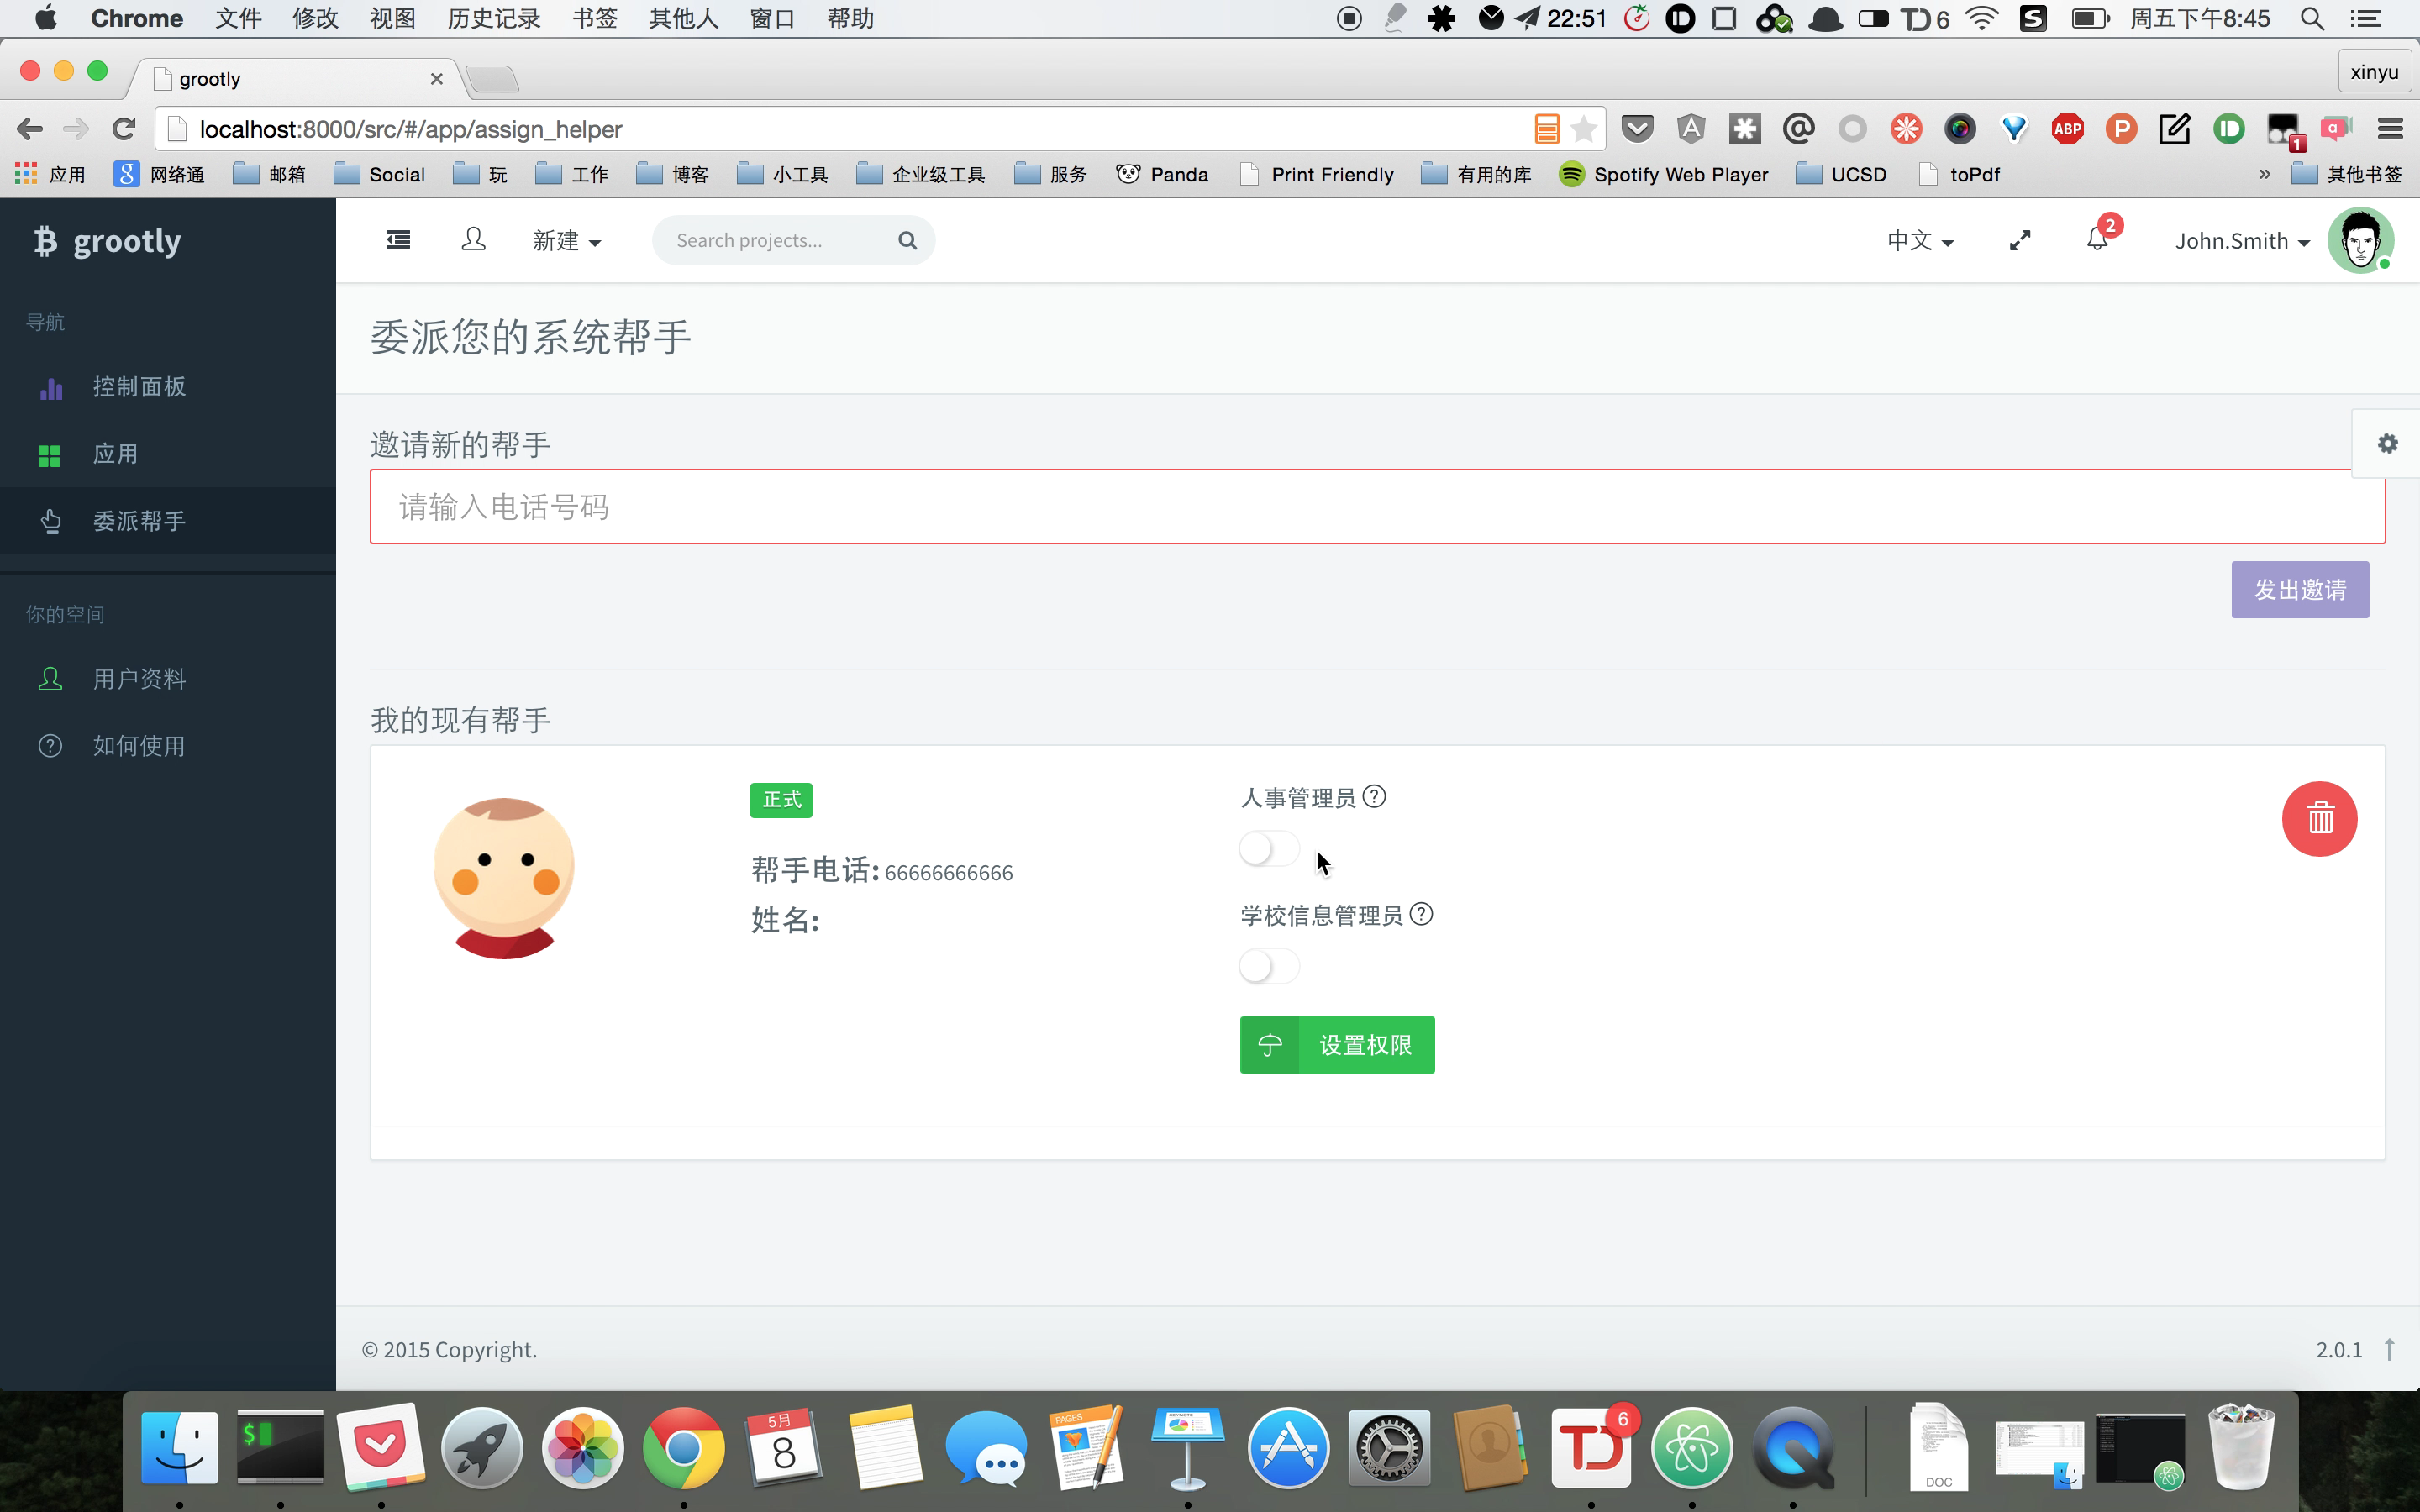
\includegraphics[width=0.7\textwidth]{helper.png}
  \figcaption{Web管理端 帮手界面}
  \label{fig: pc_helper}
\end{figure}


\end{itemize}




\section{Mobile App社交界面设计}

\begin{itemize}

\item 浏览状态界面

\begin{figure}[H]
  \centering
  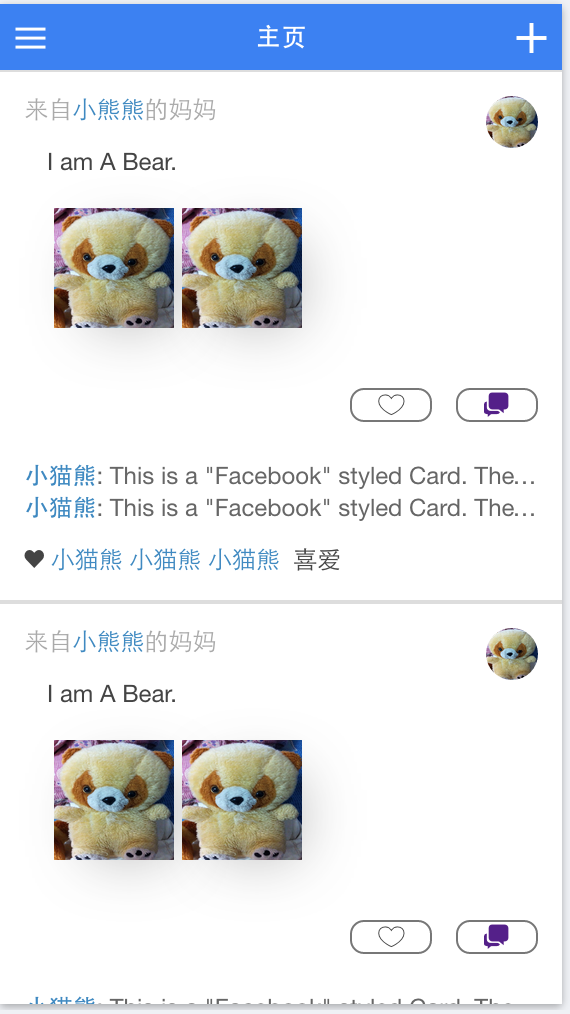
\includegraphics[width=0.3\textwidth]{app_timeline.png}
  \figcaption{App 时间线界面}
  \label{fig: app_timeline}
\end{figure}


\item 发布状态界面

\begin{figure}[H]
  \centering
  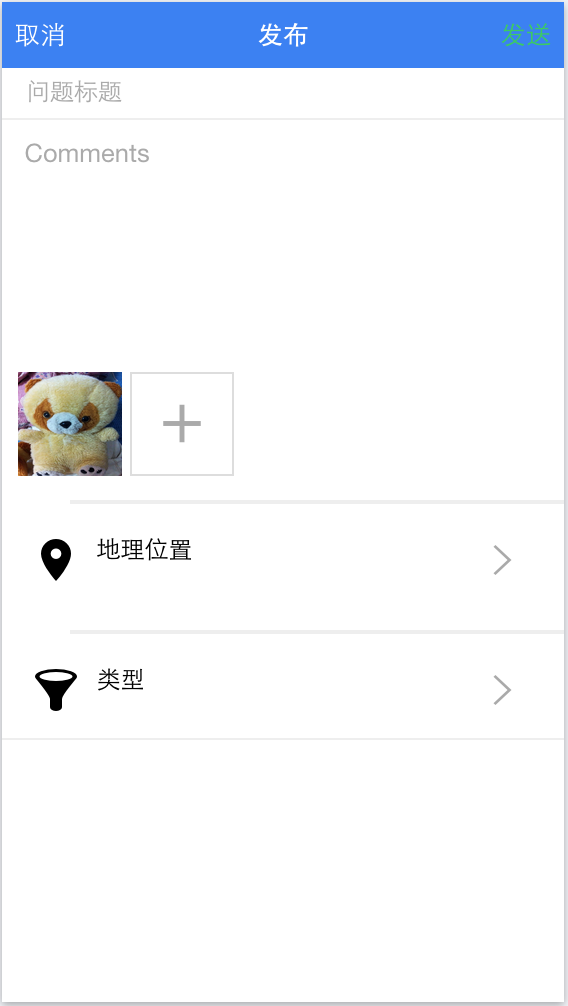
\includegraphics[width=0.3\textwidth]{app_post.png}
  \figcaption{App 发布状态界面}
  \label{fig: app_post}
\end{figure}



\item 聊天界面


\begin{figure}[H]
  \centering
  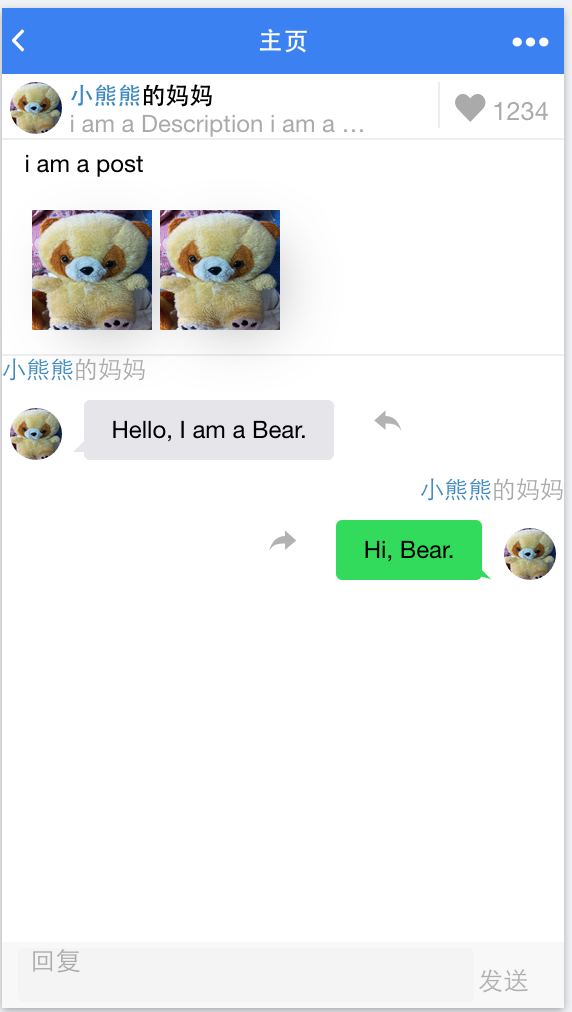
\includegraphics[width=0.3\textwidth]{app_chat.png}
  \figcaption{App 聊天界面}
  \label{fig: app_chat}
\end{figure}


\item 我的班级和学校界面


\begin{figure}[H]
  \centering
  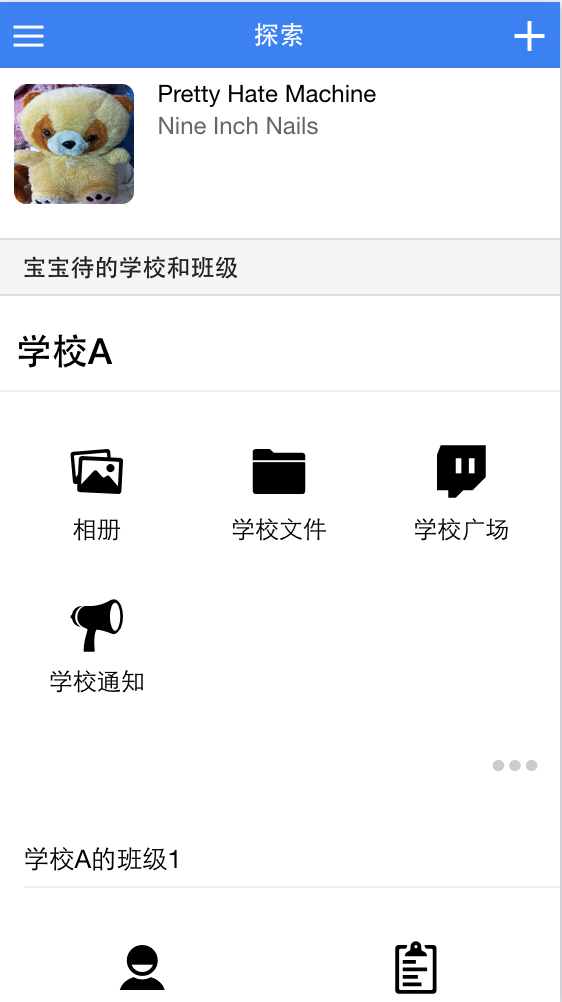
\includegraphics[width=0.3\textwidth]{app_class.png}
  \figcaption{App 我的班级和学校界面}
  \label{fig: app_class}
\end{figure}


\end{itemize}
